
\chapter{应用：曲线}
\label{ch:curves}

现在，我们要用已经建立起来的理论来研究一些具体的东西——\trCurve。在本章中，我们始终假设所有\trCurve{}都是域 $k$ 上射影的、几何整的、正则的\trCurve。我们有时会追加「$k$ 代数闭」这一假设。多数人乐于在代数闭域上工作，这些读者可以无视「几何地」这个副词。

要理解\trCurve，我们当然用不着已经建立起来的那整套庞大的机器；但有了我们业已获得的视角，这套展开是相当干净的。我们将需要的关键配料如下。我们要用到\trMorphism{}为\trClosedEmbedding{}的一个判别法，其证明在 \S19.1。我们要用到\trSerreDuality{}这个「黑箱」（其证明见第 29 章）。在 \S19.2 中，我们利用这些背景观察寥寥几条有用的事实，并将反复使用它们。最后，在把它们应用于理解各种\trGenus{}的\trCurve{}的过程中，我们会以动手的方式发展\trHyperelliptic\trCurve{}的理论（\S19.5），特别地证明\trRiemann--\trHurwitz{}公式的一个特例。

如果你没有多少先前的阅读就直接跳进本章，应当跳过 \S19.1，把\mbox{定理~19.1.1} 当作黑箱。视你的背景而定，你可能还想连 \S19.2 也一并跳过，把那些「关键工具」当作黑箱。


\section{态射为\trClosedEmbedding{}的一个判别法}

我们将反复使用一个判定\trMorphism{}何时为\trClosedEmbedding{}的判别法，它并非\trCurve{}所独有。在陈述它之前，我们先回忆一些关于\trClosedEmbedding{}的事实。设 $\pi\colon X\to Y$ 是一个\trClosedEmbedding。那么 $\pi$ 是\trProjective{}的，并且在点上单射。仅凭这些还不足以保证它是\trClosedEmbedding{}——\trCusp{}的\trNormalization{}这个例子（图~\ref{fig:cusp-normalization}）便表明了这一点。另一个例子是下面这道练习。

\textbf{19.1.A.（练习：\trFrobenius；参看 \S8.3.Q）}\quad 证明：由 $x\mapsto x^{p}$ 给出的 $\pi\colon\mathbb{A}^1_{\mathbb{F}_p}\to\mathbb{A}^1_{\mathbb{F}_p}$ 在点上双射，并且在\trClosedPoint{}上诱导\trResidueField{}的同构，然而它并不是\trClosedEmbedding。

为了使一个\trMorphism{} $\pi$ 是\trClosedEmbedding，你所需要的附加信息是：切映射在一切\trClosedPoint{}处都是单射。

\textbf{19.1.B.（练习）}\quad 证明（直接证明，不要援引\mbox{定理~19.1.1}）：在上文描述的两个例子（\trCusp{}的\trNormalization{}与\trFrobenius{}态射）中，切映射在一切\trClosedPoint{}处都\emph{不}单射。

\textbf{19.1.1.\ \trhTheorem。}\ ——\ \emph{设 $k=\overline{k}$，而 $\pi\colon X\to Y$ 是有限型 $k$-\trScheme{}之间的一个\trProjective\trMorphism，它在\trClosedPoint{}上单射，并且在\trClosedPoint{}处的\trTangentVector{}上单射。那么 $\pi$ 是一个\trClosedEmbedding。}

逆命题是显然的，所以你应当把这个结果当作「当且仅当」来用。

（注记：对于代数闭域上的有限型概形这一情形，「在\trClosedPoint{}处的\trTangentVector{}上单射」等价于「\trUnramified」；见\mbox{练习~21.7.E}。我们将在 \S21.7 中定义\trUnramified。）

例子 $\Spec\mathbb{C}\to\Spec\mathbb{R}$ 表明：在\mbox{定理~19.1.1} 中我们确实需要「$k$ 是\trAlgClosed{}的」这条假设。对\trAlgClosedField{}过敏的读者也请留心，因为我们将用它来证明关于 $k$ 上\trCurve{}的一些结果，其中 $k$ \emph{未必}是\trAlgClosed{}的（另见\mbox{练习~10.2.K} 与\mbox{练习~19.1.F}）。

我们还需要「该\trMorphism{}是\trProjective{}的」这条假设，图~\ref{fig:projectivity-node-example} 的例子表明了这一点。这个例子是\trNode{}的\trNormalization{}，只是我们把\trNode{}的诸原像之一擦去了。我们把 $\mathbb{A}^1$ 映入平面，使得它的像是一条带一个\trNode{}的\trCurve。然后我们考虑丢弃\trNode{}的一个原像之后所得的\trMorphism。此时这个\trMorphism{}在点上单射，并且在\trTangentVector{}上也单射，但它不是\trClosedEmbedding{}。（在\trDifferentialGeometry{}的世界里，它之所以算不得嵌入，是因为这个映射不给出到其像上的\trHomeomorphism。）

\begin{figure}[htbp]
\centering
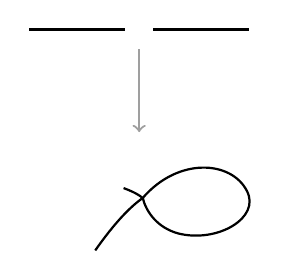
\begin{tikzpicture}[scale=0.9,line width=0.8pt]
  \draw[line width=1.2pt] (-1.55,2.40) -- (-0.20,2.40);
  \draw[line width=1.2pt] (0.20,2.40) -- (1.55,2.40);
  \draw[gray!75,->] (0,2.12) -- (0,0.95);
  \draw (0.05,0.02) .. controls (0.55,0.60) and (1.30,0.55) .. (1.52,0.12)
        .. controls (1.72,-0.26) and (1.10,-0.62) .. (0.55,-0.48)
        .. controls (0.26,-0.40) and (0.10,-0.18) .. (0.05,0.02);
  \draw (-0.22,0.16) .. controls (-0.06,0.10) and (0.00,0.06) .. (0.05,0.02)
        .. controls (-0.12,-0.10) and (-0.34,-0.32) .. (-0.62,-0.72);
\end{tikzpicture}
\caption{（图~\ref{fig:normalization-nodal-cubic} 的变体）\mbox{定理~19.1.1} 中的\trProjective{}性假设不能去掉。（依原书手绘图重绘。）}\label{fig:projectivity-node-example}
\end{figure}

\mbox{定理~19.1.1} 看上去根本上是关于\trVariety{}的一个陈述，但其实并不是。我们将把它化归为下面的结果。

\textbf{19.1.2.\ \trhTheorem。}\ ——\ \emph{设 $\pi\colon X\to Y$ 是\trNoetherian{}\trScheme{}之间的一个\trFinite\trMorphism，它在 $Y$ 的每一点处的次数（\S14.3.4）为 $0$ 或 $1$。那么 $\pi$ 是一个\trClosedEmbedding。}

\textbf{19.1.C.（练习）}\quad 设 $\pi\colon X\to Y$ 是一个\trFinite\trMorphism，它在 $Y$ 的每一点处的次数为 $0$ 或 $1$。证明：$\pi$ 在点上单射（容易）。若 $p\in X$ 是任一点，证明 $\pi$ 诱导\trResidueField{}的同构 $\kappa(\pi(p))\overset{\sim}{\longrightarrow}\kappa(p)$。证明 $\pi$ 诱导\trTangentSpace{}之间的一个单射。于是，\mbox{定理~19.1.1} 的几条关键假设便都隐含在\mbox{定理~19.1.2} 的假设之中了。

\textbf{19.1.3.}\ \emph{\mbox{定理~19.1.1} 到\mbox{定理~19.1.2} 的化归。}\quad 「是\trClosedEmbedding」这一性质在靶上是局部的，故我们不妨假设 $Y$ 是\trAffine{}的，比如说 $\Spec B$。

接下来我断言：$\pi$ 具有\trFinite\trFiber——而不只是在\trClosedPoint{}之上\trFiber{}有限：\trProjective\trMorphism{}的纤维维数是\trUpperSemicontinuous{}的（\mbox{练习~18.1.B}，或\mbox{定理~12.4.3(b)}），于是纤维维数至少为 $1$ 的那个\trLocus{}是一个\trClosedSubset，从而若它非空，就必然含有 $Y$ 的一个\trClosedPoint。于是，任一点之上的\trFiber{}都是该点之上的维数 $0$ 的有限型\trScheme，因而是个\trFinite{}集。

于是 $\pi$ 是一个带\trFinite\trFiber{}的\trProjective\trMorphism，从而由\mbox{定理~18.1.6} 是\trFinite{}的。

\textbf{19.1.D.（练习）}\quad 证明：$\pi$ 的次数在 $Y$ 的一切\trClosedPoint{}处都至多为 $1$。（提示一：这里你将用到「在\trTangentVector{}上单射」这条假设。提示二：到 $\Spec\overline{k}$ 的\trFinite\trMorphism{}都有哪些？）

但\trFinite\trMorphism{}的次数是\trUpperSemicontinuous{}的（\S14.3.4），故在一切点处都至多为 $1$（你看出这是为什么了吗？）。这样我们便证明了：\mbox{定理~19.1.1} 可以由\mbox{定理~19.1.2} 推出。

\textbf{19.1.4.}\ \emph{\mbox{定理~19.1.2} 的证明。}\quad 这个问题在 $Y$ 上是局部的，故我们不妨假设 $Y$ 是\trAffine{}的，比如说 $Y=\Spec B$。于是 $X$ 也是\trAffine{}的，比如说 $\Spec A$，而 $\pi$ 对应于一个\trRingMorphism{} $B\to A$。我们想证明这是一个环的满射，或者（等价地）$B$-\trModule{}的满射。令 $K$ 是这个 $B$-\trModule{}态射的\trCokernel：
\begin{equation*}\tag{19.1.4.1}\label{eq:criterion-cokernel-sequence}
B\longrightarrow A\longrightarrow K\longrightarrow 0.
\end{equation*}
我们想证明 $K=0$。只须证明：对 $B$ 的任意\trMaximalIdeal{} $\mathfrak{n}$ 都有 $K_{\mathfrak{n}}=0$。（你还记得这是为什么吗？）把 \eqref{eq:criterion-cokernel-sequence} 在 $\mathfrak{n}$ 处局部化，便得到正合列
\[
B_{\mathfrak{n}}\longrightarrow A_{\mathfrak{n}}\longrightarrow K_{\mathfrak{n}}\longrightarrow 0.
\]
施加右正合函子 $\otimes_{B_{\mathfrak{n}}}(B_{\mathfrak{n}}/\mathfrak{n}B_{\mathfrak{n}})$，便得
\begin{equation*}\tag{19.1.4.2}\label{eq:criterion-tensor-cokernel-sequence}
B_{\mathfrak{n}}/\mathfrak{n}B_{\mathfrak{n}}\overset{\alpha}{\longrightarrow}A_{\mathfrak{n}}/\mathfrak{n}A_{\mathfrak{n}}\longrightarrow K_{\mathfrak{n}}/\mathfrak{n}K_{\mathfrak{n}}\longrightarrow 0.
\end{equation*}
现在 $\Spec A_{\mathfrak{n}}/\mathfrak{n}A_{\mathfrak{n}}$ 是 $[\mathfrak{n}]\in\Spec B$ 的\trSchemeTheoreticPreimage，故由假设，它要么是空的，要么映射 $\alpha$ 是同构（在这一情形，我们将会看到 $\alpha$ 原来就是剩余域的映射）。在前一情形，$A_{\mathfrak{n}}/\mathfrak{n}A_{\mathfrak{n}}=0$，从而 $K_{\mathfrak{n}}/\mathfrak{n}K_{\mathfrak{n}}=0$；在后一情形，同样有 $K_{\mathfrak{n}}/\mathfrak{n}K_{\mathfrak{n}}=0$。施加\trNakayama{}引理~8.2.9（注意 $A$ 是有限生成的 $B$-\trModule，因而 $K$ 亦然，进而 $K_{\mathfrak{n}}$ 是有限生成的 $B_{\mathfrak{n}}$-\trModule），便得 $K_{\mathfrak{n}}=0$，正如所求。\hfill$\square$

\mbox{练习~10.2.K} 可以用来把\mbox{定理~19.1.1} 的效力延伸到一般的域 $k$——不必是\trAlgClosed{}的域。下面的练习就是一个例子，示范怎么做。

\textbf{19.1.E.（练习）}\quad 用\mbox{定理~19.1.1} 证明：从 $\mathbb{P}^n_k$ 出发、相应于完全线性系 $|\OO_{\mathbb{P}^n_k}(d)|$ 的第 $d$ 次\trVeroneseEmbedding{}是一个\trClosedEmbedding。对从 $\mathbb{P}^m_k\times_{\Spec k}\mathbb{P}^n_k$ 出发的\trSegre{}嵌入做同样的事。（这只是为了练习使用这个判别法。它比我们先前的结果要弱；这两条陈述我们先前都已在任意基环上验证过——分别在\mbox{注记~9.3.8} 与 \S10.6——而现在我们只在域上验证。不过，请参看下面的\mbox{练习~19.1.F}。）

\textbf{19.1.F.（较不重要的练习）}\quad 用本节的想法证明：从 $\mathbb{P}^n_{\mathbb{Z}}$（在整数环上！）出发的第 $d$ 次\trVeroneseEmbedding{}是一个\trClosedEmbedding。（再说一次，这件事我们以前做过。这道练习只是要表明：这些方法可以轻松推广，在更一般的情形同样奏效。）


\section{一系列关键工具}

现在，我们已经准备好以一种动手的方式来理解\trCurve{}了。我们将反复使用下面这一系列关键评注；而把它们挂在嘴边、随时能信手拈来，是很要紧的。

\textbf{19.2.1.}\quad \emph{在下文中，$C$ 将是域 $k$ 上一条\trProjective{}、几何正则、\trGeometricallyIntegral{}的\trCurve，而 $\mathscr{L}$ 是 $C$ 上的一个\trInvertibleSheaf。}

\textbf{19.2.2. 提醒：\trSerreDuality。}\quad $k$ 上\trGeometricallyIrreducible{}正则的\trGenus{} $g$ \trCurve{} $C$ 上的\trSerreDuality（\mbox{定理~18.5.1}）牵涉到一个\trInvertibleSheaf{} $\omega_C$（次数为 $2g-2$，且带有 $g$ 个线性无关的截面，\mbox{练习~18.5.A}），使得对 $C$ 上任意有限\trRank{}\trLocallyFreeSheaf{} $\mathscr{F}$，当 $i=0$、$1$ 时都有 $h^i(C,\mathscr{F})=h^{1-i}(C,\omega_C\otimes\mathscr{F}^{\vee})$。（更好的说法：在那两个\trCohomology{}群之间存在一个对偶。）

\textbf{19.2.3. 负\trDegree{}\trLineBundle{}没有非零\trSection。}\quad 若 $\deg\mathscr{L}<0$，则 $h^0(C,\mathscr{L})=0$。理由：$\deg\mathscr{L}$ 是任一\trRational{}截面的零点个数减去极点个数（适当地计数）（\mbox{重要练习~18.4.C}）。若存在一个正则截面（即没有极点的截面），此时该次数必非负。把这番论证加以精化，便得到下面的结论。

\textbf{19.2.4. \trDegree{} $0$ 的\trLineBundle，以及识别它们何时是\trTrivial{}的。}\quad 若 $\deg\mathscr{L}=0$，则 $h^0(C,\mathscr{L})=0$ 或 $1$；而且若 $h^0(C,\mathscr{L})=1$，则 $\mathscr{L}\cong\OO_C$。理由：若存在一个非零截面 $s$，则它没有极点，从而也没有零点，因为 $\deg\mathscr{L}=0$。于是 $\operatorname{div}s=0$，故 $\mathscr{L}\cong\OO_C(\operatorname{div}s)=\OO_C$。（回想一下这是怎么回事；参看\mbox{重要练习~15.4.G}：$s$ 给出该\trInvertibleSheaf{}的一个\trTrivialization。对任意开集 $\mathrm{U}$\footnote{原书此处作「for any open set」，当为「for any open set U」之脱文，径补。——译者注}，我们都有自然的双射 $\Gamma(\mathrm{U},\mathscr{L})\overset{\sim}{\longleftrightarrow}\Gamma(\mathrm{U},\OO_{\mathrm{U}})$，其中从左到右的映射是 $s'\mapsto s'/s$，从右到左的映射是 $f\mapsto sf$。）反之，对几何整的射影\trVariety{}而言，$h^0(\OO)=1$。（\S11.4.7 在 $k$ \trAlgClosed{}时证明了这一点——这正是用到几何整性的地方——而\mbox{练习~18.2.H} 则证明了\trCohomology{}与基域扩张交换。）

\trSerreDuality{}把上述关于\trDegree{}至多为 $0$ 的\trLineBundle{}的诸陈述，转成了关于\trDegree{}至少为 $2g-2$ 的\trLineBundle{}的诸陈述，如下。

\textbf{19.2.5. 若\trDegree{}足够高，则我们知道 $h^0(C,\mathscr{L})$。}\quad 若 $\deg\mathscr{L}>2g-2$，则
\begin{equation*}\tag{19.2.5.1}\label{eq:h0-high-degree}
\fbox{$h^0(C,\mathscr{L})=\deg\mathscr{L}-g+1$.}
\end{equation*}
于是当 $\deg\mathscr{L}\gg 0$ 时，我们就知道 $h^0(C,\mathscr{L})$。（\emph{这很重要——要记住这一条！}）理由：$h^1(C,\mathscr{L})=h^0(C,\omega_C\otimes\mathscr{L}^{\vee})$；但 $\omega_C\otimes\mathscr{L}^{\vee}$ 的\trDegree{}为负（因为 $\omega_C$ 的\trDegree{}是 $2g-2$），于是这个\trInvertibleSheaf{}没有截面。这个结果随即由以 \eqref{eq:riemann-roch-h0-h1} 的面目出现的\trRiemannRoch{}定理得到。

\textbf{19.2.A.（有用练习：在\trDegree{} $2g-2$ 的诸\trLineBundle{}中认出 $\omega_C$）}\quad 设 $\mathscr{L}$ 是一个\trDegree{}为 $2g-2$ 的\trInvertibleSheaf。证明：它有 $g-1$ 或 $g$ 个截面，而且它有 $g$ 个截面，当且仅当 $\mathscr{L}\cong\omega_C$。

\textbf{19.2.B.（练习）}\quad 设 $C$ 是一条\trGenus{} $g>1$ 的\trCurve，所在的域 $k$ 不必\trAlgClosed。证明：$C$ 有一个在基域上\trDegree{}至多为 $2g-2$ 的\trClosedPoint。（作为对照：当 $g=1$ 时，对任意 $n$，都存在 $\mathbb{Q}$ 上的一条\trGenus{} $1$ \trCurve，它没有\trDegree{}小于 $n$ 的点，[MO286390]\footnote{译注：[MO286390] 指 MathOverflow 问答第 286390 号。}！）

\textbf{19.2.6. 用一个（\trDegree{} $1$ 的）点扭转 $\mathscr{L}$，至多把 $h^0$ 改变 $1$。}\quad 设 $p$ 是任意一个\trDegree{}为 $1$ 的\trClosedPoint（即 $p$ 的\trResidueField{}是 $k$）。则 $h^0(C,\mathscr{L})-h^0(C,\mathscr{L}(-p))=0$ 或 $1$。（用一个\trDivisor{}扭转 $\mathscr{L}$，比如 $\mathscr{L}(-p)$，曾定义于 \S15.4.17。）理由：考察 $0\to\OO_C(-p)\to\OO_C\to\OO|_{p}\to 0$；与 $\mathscr{L}$ 作张量（由于 $\mathscr{L}$ \trLocallyFree，这是正合的），便得到
\[
0\longrightarrow \mathscr{L}(-p)\longrightarrow \mathscr{L}\longrightarrow \mathscr{L}|_{p}\longrightarrow 0.
\]
那么 $h^0(C,\mathscr{L}|_{p})=1$，于是\trCohomology{}的\trLongExactSequence{}开头为
\[
0\longrightarrow \mathrm{H}^0(C,\mathscr{L}(-p))\longrightarrow \mathrm{H}^0(C,\mathscr{L})\longrightarrow \mathrm{H}^0(C,\mathscr{L}|_{p}),
\]
我们便大功告成。

\textbf{19.2.7. $\mathscr{L}$ 无基点的判别法。}\quad 就本条评注而言，设 $k$ \trAlgClosed，从而\emph{一切}\trClosedPoint{}在 $k$ 上的\trDegree{}都是 $1$。那么，若对\emph{一切}\trClosedPoint{} $p$ 都有 $h^0(C,\mathscr{L})-h^0(C,\mathscr{L}(-p))=1$，则 $\mathscr{L}$ \trBasePointFree，从而诱导出一个从 $C$ 到\trProjectiveSpace{}的\trMorphism（\mbox{定理~15.2.2}）。理由：任给 $p$，我们的等式表明，存在 $\mathscr{L}$ 的一个在 $p$ 处不消失的截面——于是按定义，$p$ 不是 $\mathscr{L}$ 的\trBasePoint。

\textbf{19.2.8.}\quad 接着，设 $p$ 与 $q$ 是互不相同的两个（闭）点，\trDegree{}皆为 $1$。则 $h^0(C,\mathscr{L})-h^0(C,\mathscr{L}(-p-q))=0$、$1$ 或 $2$（把\mbox{注记~19.2.6} 的论证重复两遍即可）。若 $h^0(C,\mathscr{L})-h^0(C,\mathscr{L}(-p-q))=2$，则必然
\begin{equation*}\tag{19.2.8.1}\label{eq:separating-points-equality}
h^0(C,\mathscr{L})=h^0(C,\mathscr{L}(-p))+1=h^0(C,\mathscr{L}(-q))+1=h^0(C,\mathscr{L}(-p-q))+2.
\end{equation*}
这时，线性系 $\mathscr{L}$ 分离点 $p$ 与 $q$，也就是说，到\trProjectiveSpace{}的相应映射 $f$ 满足 $f(p)\ne f(q)$。理由：\trProjectiveSpace{}中存在一张\trHyperplane{}经过 $f(q)$ 而不经过 $f(p)$；等价地，$\mathscr{L}$ 存在一个在 $q$ 处消失而在 $p$ 处不消失的截面。这正是 \eqref{eq:separating-points-equality} 中最后一个等式的内容。

\textbf{19.2.9.}\quad 由与上文相同的论证，若 $p$ 是一个\trDegree{}为 $1$ 的（闭）点，则 $h^0(C,\mathscr{L})-h^0(C,\mathscr{L}(-2p))=0$、$1$ 或 $2$。我宣称：若这个值是 $2$，则相应于 $\mathscr{L}$ 的映射（由上文已知它在 $p$ 处无基点）分离 $p$ 处的切向量。为了证明这一点，我们需要证明余切映射是满射。而要证明到一个一维\trVectorSpace{}的满射性，只须证明该映射非零。于是，只须在靶上找到一个在 $p$ 的像处消失的函数，使得其拉回是一个在 $p$ 处消失到 $1$ 阶而非 $2$ 阶的函数。换言之，我们想要的是 $\mathscr{L}$ 的一个在 $p$ 处消失到 $1$ 阶而不消失到 $2$ 阶的截面。而这正是陈述 $h^0(C,\mathscr{L}(-p))-h^0(C,\mathscr{L}(-2p))=1$ 的内容。

\textbf{19.2.10. $\mathscr{L}$ 为极丰富的判别法。}\quad 把上文的一些评注结合起来：设 $C$ 是代数闭域 $k$ 上的一条\trCurve，而 $\mathscr{L}$ 是一个\trInvertibleSheaf，使得对\emph{一切}\trClosedPoint{} $p$ 与 $q$——\emph{不必互不相同}——都有 $h^0(C,\mathscr{L})-h^0(C,\mathscr{L}(-p-q))=2$；那么 $\mathscr{L}$ \emph{给出一个到\trProjectiveSpace{}的\trClosedEmbedding}，因为它分离点与切向量：由\mbox{定理~19.1.1}。

\textbf{19.2.C.（练习）}\quad 假设 $k$ \trAlgClosed，于是前一条评注适用。证明：$C\setminus\{p\}$ 是\trAffine{}的。提示：证明若 $j\gg 0$，则 $\OO(jp)$ 无基点，并且至少有两个线性无关的截面，其中之一的\trDivisor{}是 $jp$。用这两个截面映射到 $\mathbb{P}^1$，使得 $\infty$ 的集合论原像是 $p$。论证该映射是\trFinite{}的，而 $C\setminus\{p\}$ 是 $\mathbb{A}^1$ 的原像。（这一论证的一个平凡变体表明：当 $n>0$ 时，$C\setminus\{p_1,\dots,p_n\}$ 是\trAffine{}的。）

\textbf{19.2.11. 有力结论：$\mathscr{L}$ 无基点与极丰富的数值判别法。}\quad 我们可以把上述讨论的很大一部分合并起来，给出下面这条有用的事实。若 $k$ \trAlgClosed，则 $\deg\mathscr{L}\ge 2g$ 蕴涵 $\mathscr{L}$ \trBasePointFree（从而确定一个到\trProjectiveSpace{}的\trMorphism）。此外，$\deg\mathscr{L}\ge 2g+1$ 蕴涵：对 $\mathscr{L}$ 的任意一组截面基 $s_0,\dots,s_{\deg\mathscr{L}-g}$，由 $[s_0,\dots,s_{\deg\mathscr{L}-g}]$ 给出的\trMorphism{}事实上是一个到 $\mathbb{P}^{\deg\mathscr{L}-g}$ 的\trClosedEmbedding（于是 $\mathscr{L}$ 是\trVeryAmple{}的）。记住这一条！

\textbf{19.2.D.（练习：关于 $\bar{k}$ 上射影、正则、整的曲线，\trAmple{}＝正\trDegree）}\quad 证明：$\bar{k}$ 上一条射影、正则、整的曲线上的\trInvertibleSheaf{} $\mathscr{L}$ 是\trAmple{}的，当且仅当 $\deg\mathscr{L}>0$。

（借下文\mbox{练习~19.2.E} 之助，这一点可以推广到一般域上的曲线。）于是，曲线上\trLineBundle{}的\trAmpleness{}有一条简单粗暴的纯数值判别法。这一点可以推广到更高维数的射影\trVariety；它称作\emph{丰富性的\trNakai--\trMoishezon{}判别法}（Nakai--Moishezon criterion for ampleness），见\mbox{定理~20.4.1}。

\textbf{19.2.E.（练习：向非\trAlgClosed{}域的扩张）}\quad 证明：即使去掉 $k$ \trAlgClosed{}这一假设，\S19.2.11 中的诸陈述也依然成立。（提示：要证明关于某条\trCurve{} $C$ 与某个\trLineBundle{} $\mathscr{L}$ 的两条事实中的一条，改为考察 $C\times_{\Spec k}\Spec\bar{k}$。然后证明：若 $\mathscr{L}$ 在这里的拉回具有能给出两条所欲性质之一的截面，则「底下」就有具有同样性质的截面。你或许想动用我们已经用过的事实，例如：无基点性独立于基域的任何扩张（\mbox{练习~18.2.I}）；或者，$k$ 上的仿射态射为\trClosedEmbedding{}这一性质，在作 $k$ 的扩张之后成立，当且仅当它在扩张之前成立（\mbox{练习~10.2.K}）。）

\textbf{19.2.F.（练习：扩充\mbox{练习~19.2.D}）}\quad 设 $\mathscr{L}$ 是（域 $k$ 上的）一条\trProjective{}、几何正则、\trGeometricallyIntegral{}\trCurve{} $C$ 上的一个\trInvertibleSheaf。证明：$\mathscr{L}$ 是\trAmple{}的，当且仅当 $\deg\mathscr{L}>0$。提示：借\mbox{练习~10.2.K} 之助，化归到 $k$ \trAlgClosed{}的情形。

\textbf{19.2.G.（练习）}\quad 设 $C$ 是一条\trCurve（照本节的惯例，即取 \S19.2.1 意义下的曲线），而 $p\in C$ 是一个\trClosedPoint。证明：$C\setminus\{p\}$ 是\trAffine{}的。提示：\mbox{练习~19.2.F}。

现在，我们已整装待发，要带上这些事实到 \S19.3 中大干一场了。

\textbf{19.2.12.}\ \hard\ \textbf{\trhRemark：\trProper{}\trCurve{}是\trProjective{}的。}

（在 \S19.2 的这最后一部分中，我们不再假设诸曲线是光滑的，甚至不再假设它们正则或既约。）我们此处的讨论，连同\trSerre{}的丰富性上同调判别法（\S18.8），是证明「域上每条\trProper{}\trCurve{}都是\trProjective{}的」这一结果的关键配料。

\textbf{19.2.H.（练习）}\quad 证明：每条\trReduced{}的\trProper{}\trCurve{} $C$ 都是\trProjective{}的。提示：在 $C$ 的每个\trIrreducibleComponent{}上选一个正则点，并令 $\mathscr{L}$ 为相应的\trInvertibleSheaf。我们盼着 $\mathscr{L}$ 会是\trAmple{}的。回想：$C$ 上的一个\trLineBundle{}是\trAmple{}的，若它到 $C$ 的\trNormalization{}上的拉回是\trAmple{}的（\mbox{棘手练习~18.8.C}）。所以请证明：到\trNormalization{}上的拉回是\trAmple{}的。

\textbf{19.2.I.（练习）}\quad 先在 $C$ 上找出一个你将证明为\trAmple{}的\trInvertibleSheaf，然后利用\mbox{练习~18.8.A} 证明：每条\trProper{}（不必\trReduced）的\trCurve{} $C$ 都是\trProjective{}的。

\textbf{19.2.J.（练习）}\quad 证明：射影曲线上的一个\trLineBundle{}是\trAmple{}的，当且仅当它在每个分量上的\trDegree{}都是正的。


\section{\trGenus{} $0$ 的\trCurve}

现在，我们已经准备好（以某种形式）回答这样一个问题了：\trGenus{} $0$ 的\trCurve{}都是些什么？

在 \S7.5.10 中，我们见过一条（域 $k$ 上的）\trGenus{} $0$ \trCurve，它并不同构于 $\mathbb{P}^1$：即 $\mathbb{P}^2_\mathbb{R}$ 中的 $x^2+y^2+z^2=0$。（由 \eqref{eq:genus-plane-curve}，它的\trGenus{}为 $0$。）我们已经观察到，这条曲线并不同构于 $\mathbb{P}^1_\mathbb{R}$，因为它没有 $\mathbb{R}$-\trValuedPoint。另一方面，我们还不曾在\trAlgClosedField{}上见过具有这种性质的\trGenus{} $0$ \trCurve。这绝非巧合：$k$-\trValuedPoint{}的缺失，正是一条\trGenus{} $0$ \trCurve{}成为 $\mathbb{P}^1$ 的唯一障碍。

\textbf{19.3.1.\ \trhProposition。}\ ——\ \emph{设 $C$ 的\trGenus{}为 $0$，且 $C$ 有一个 $k$-\trValuedPoint（\trDegree{} $1$）。那么 $C\cong\mathbb{P}^1_k$。}

于是我们看到：\trAlgClosedField{}上的一切\trGenus{} $0$（\trIntegral、\trRegular、\trProjective）\trCurve{}都同构于 $\mathbb{P}^1$。

\emph{证明。}\quad 设 $p$ 为那个点，并考虑 $\mathscr{L}=\OO_C(p)$。于是 $\deg\mathscr{L}=1$，故我们可以应用上文已知的结果：其一，$h^0(C,\mathscr{L})=2$（\mbox{注记~19.2.5}）；其二，这两个\trSection{}给出一个到 $\mathbb{P}^1_k$ 的\trClosedEmbedding（\mbox{注记~19.2.11}，经\mbox{练习~19.2.E} 扩充）。但是，一条\trCurve{}到\trIntegral\trCurve{} $\mathbb{P}^1_k$ 之内的\trClosedEmbedding{}只能是同构！\hfill$\square$

附带一提，\mbox{命题~19.3.1} 蕴涵：$\mathbb{P}^2_\mathbb{R}$ 中的 $x^2+y^2+z^2=0$ 在 $\mathbb{R}$ 上没有\emph{次数 $1$ 的\trLineBundle}——否则，我们只须把上面的论证施加到相应的\trLineBundle{}上就行了。这个例子向我们表明：在一个非\trAlgClosed{}的域上，可以存在不同构于 $\mathbb{P}^1_k$ 的\trGenus{} $0$ \trCurve。下面这个结果让我们也能把它们亲手抓到。

\textbf{19.3.2.\ \trhClaim。}\ ——\ \emph{一切\trGenus{} $0$ \trCurve{}都可以描述为 $\mathbb{P}^2_k$ 中的\trConic。}

\emph{证明。}\quad 任何\trGenus{} $0$ \trCurve{}都有一个\trDegree{}为 $-2$ 的\trLineBundle——即\trCanonical{}层 $\omega_C$。于是任何\trGenus{} $0$ \trCurve{}都有一个\trDegree{}为 $2$ 的\trLineBundle：$\mathscr{L}=\omega_C^{\vee}$。我们应用\mbox{练习~19.2.E}：$\deg\mathscr{L}=2\ge 2g+1$，故这个\trLineBundle{}给出一个\trClosedEmbedding{} $\iota\colon C\hookrightarrow\mathbb{P}^2$。\mbox{练习~18.6.H} 保证该像作为\trClosedSubscheme{}的\trDegree{}为 $2$；但我们还没有完全证明，这条\trCurve{}可以由单个\trDegree{} $2$ 的齐次多项式割出。（这件事比你想的更微妙——在读下去之前，你不妨先试着自己论证一番。）我们有同构 $\Sym^2\mathrm{H}^0(\mathbb{P}^2,\OO(1))\overset{\sim}{\longrightarrow}\mathrm{H}^0(\mathbb{P}^2,\OO(2))$（两边都是三个变量的齐次二次多项式）。考察映射 $\Sym^2\mathrm{H}^0(C,\mathscr{L})\to\mathrm{H}^0(C,\mathscr{L}^{\otimes 2})$，由 \eqref{eq:h0-high-degree}，它是从一个维数为 $6$ 的\trVectorSpace{}到一个维数为 $5$ 的\trVectorSpace{}的映射。这个映射有非平凡的\trKernel，故 $\iota(C)$ \trSchemeTheoretic{}地含于 $V(f)$ 之中，其中 $f$ 为某个齐次\trConic。

\textbf{19.3.A.（练习）}\quad 用\mbox{练习~18.6.E} 证明：$\iota(C)$ \trSchemeTheoretic{}地等于 $V(f)$，从而完成上述证明。

\begin{flushright}
$\square$
\end{flushright}

\textbf{19.3.B.（练习）}\quad 设 $C$ 是一条\trGenus{} $0$ \trCurve（\trProjective、\trGeometricallyIntegral，且\trRegular）。证明：$C$ 有一个\trDegree{}至多为 $2$ 的点。（点的\trDegree{}曾定义于 \S5.3.8。）

\S7.5.9 中所呈现的、用几何手段寻找勾股三元组的方法，看上去颇为不同，但其实是一回事。当时有一条\trGenus{} $0$ \trCurve{} $C$（一条平面\trConic），带有一个 $k$-\trValuedPoint{} $p$，而我们证明了它同构于 $\mathbb{P}^1_k$。用以证明该同构的\trLineBundle{}并不是\trDegree{} $1$ 的\trLineBundle{} $\OO_C(p)$；而是\trDegree{} $1$ 的\trLineBundle{} $\OO_{\mathbb{P}^2}(1)|_C\otimes\OO_C(-p)$。


\section{正\trGenus{}\trCurve{}产生的经典几何}

后文我们会用到下面的\trhProposition{}与\trhCorollary，而我们也以此为由头，从现代的立场重访一些非常经典的几何。

\textbf{19.4.1.\ \trhProposition。}\ ——\ \emph{回想本章的\trStandingHypothesis（\S19.2.1）：$C$ 是域 $k$ 上一条\trProjective、几何正则、\trGeometricallyIntegral{}的\trCurve。设 $C$ 不同构于 $\mathbb{P}^1_k$（对其\trGenus{}不作任何假设），且 $\mathscr{L}$ 是一个\trDegree{}为 $1$ 的\trInvertibleSheaf。则 $h^0(C,\mathscr{L})<2$。}

\emph{证明。}\quad 我们本可以仿照\mbox{命题~19.3.1} 来证明它（读者也不妨一试）。但我们改为「徒手」证明，因为\mbox{命题~19.3.1} 要用到\trSerreDuality，而我们要到第 29 章才会证明它（况且它也很难），我们想强调：这个结果用不着\trSerreDuality。此外，有些读者或许从未读过任何关于\trSerreDuality{}的内容，也照样能读懂这个论证。

假设陈述不真，并设 $s_1$ 与 $s_2$ 为两个（相互独立的）\trSection。由于 $s_i$ 的零点\trDivisor{}的\trDegree{}就是 $\mathscr{L}$ 的\trDegree，故二者各自在单独一点 $p_i$ 处消失（消失到 $1$ 阶）。

现在，$p_1\ne p_2$。（否则，若 $p_1=p_2$，则 $s_1/s_2$ 既无极点又无零点，于是由代数\trHartogs{}引理——见 \S13.5.20——它是一个可逆函数，而借助 \S11.4.7（在基变换到 $\bar{k}$ 之后）它又是一个常值函数。这与 $s_1$ 与 $s_2$ 的线性无关性矛盾。）

于是 $s_1$ 与 $s_2$ 生成一个\trBasePointFree\trLinearSystem，从而我们便有一个诱导出的\trMorphism{} $C\to\mathbb{P}^1$。这是一个从一个正则\trCurve{}到另一个正则\trCurve{}的\trFinite、\trDegree{} $1$ 的\trMorphism（\mbox{练习~18.4.E}），从而诱导一个\trDegree{} $1$ 的\trFunctionField{}扩张，亦即\trFunctionField{}的同构，而这意味着两条\trCurve{}同构（参看\mbox{定理~16.3.3}）。但我们已假设 $C$ 不同构于 $\mathbb{P}^1_k$，故得出矛盾。\hfill$\square$

\textbf{19.4.2.\ \trhCorollary。}\ ——\ \emph{若 $C$ 是 $k$ 上一条\trProjective、几何正则、\trGeometricallyIntegral{}的\trCurve，不同构于 $\mathbb{P}^1_k$，而 $p$ 与 $q$ 是两个\trDegree{} $1$ 的点，则 $\OO_C(p)\cong\OO_C(q)$ 当且仅当 $p=q$。}

\textbf{19.4.A.（练习）}\quad 证明这一条。（可能有用：证明／使用：$\OO_C(p)$ 有一个整体\trSection{} $s$，使得 $\operatorname{div}(s)=p$。）

\textbf{19.4.B.（练习）}\quad 证明：若 $k$ \trAlgClosed，则 $C$ 具有\trGenus{} $0$，当且仅当一切\trDegree{} $0$ 的\trLineBundle{}都是\trTrivial{}的。

\textbf{19.4.C.（练习）}\quad 设 $C$ 是一条\trDegree{}为 $e>2$ 的\trRegular{}平面\trCurve，而 $D_1$ 与 $D_2$ 是两条\trDegree{}同为 $d$ 且均不包含 $C$ 的平面\trCurve。由平面曲线的\trBezout{}定理（\S18.6.4），$D_i$ 与 $C$ 相交于 $de$ 个点（按「正确」的方式计数）。设 $D_1$ 与 $D_2$ 在其中 $de-1$ 个「相同的点」处与 $C$ 相交，此外各另交一点。证明：余下的那些点也相同。更精确地说，设 $C$ 上有一个\trDegree{}为 $de-1$ 的\trDivisor{} $E$，以及两个\trDegree{}为 $1$ 的（$k$-\trValuedPoint）点 $p_1$ 与 $p_2$，使得 $D_i\cap C=E+p_i$（作为 $C$ 上的\trDivisor）。证明：$p_1=p_2$。（$d=e=3$ 的情形即\trChasles{}定理，并且是\trCayleyBacharach{}定理的第一个情形；见 [EGH]。）

作为\mbox{练习~19.4.C} 的一项有趣应用，我们可以证明两个经典结果。为方便起见，在这番讨论中我们将假设 $k$ \trAlgClosed，尽管这个假设很容易去掉。

\textbf{19.4.3.\ \trPappus{}定理（亚历山大里亚的\trPappus）。}\ ——\ （见图~\ref{fig:pappus}。）\emph{设 $\ell$ 与 $m$ 是平面内两条不同的直线，$\alpha$、$\beta$、$\gamma$ 是 $\ell$ 上三个互不相同的点，而 $\alpha'$、$\beta'$、$\gamma'$ 是 $m$ 上三个互不相同的点，并且这六个点都不同于 $\ell\cap m$。那么点 $x=\overline{\alpha\beta'}\cap\overline{\alpha'\beta}$、$y=\overline{\alpha'\gamma}\cap\overline{\alpha\gamma'}$\footnote{原书此处作『$\overline{\alpha\gamma}\cap\overline{\alpha\gamma'}$』，当为『$\overline{\alpha'\gamma}\cap\overline{\alpha\gamma'}$』之误，径改。——译者注}、$z=\overline{\beta\gamma'}\cap\overline{\beta'\gamma}$ 共线。}

\trPascal{}的「神秘六边形」定理是\trPascal{}在 16 岁时发现的。（16 岁那年，你在忙些什么？）

\textbf{19.4.4.\ \trPascal{}的「神秘六边形」定理。}\ ——\ （见图~\ref{fig:pascal}。）\emph{若六边形 $\alpha\gamma'\beta\alpha'\gamma\beta'$ 内接于一条光滑\trConic{} $K$，而把三对对边两两延长直至相交，则三个交点 $x=\overline{\alpha\beta'}\cap\overline{\alpha'\beta}$、$y=\overline{\alpha'\gamma}\cap\overline{\alpha\gamma'}$、$z=\overline{\beta\gamma'}\cap\overline{\beta'\gamma}$ 共线。}

\trPappus{}定理可以看成\trPascal{}定理的一个退化：二次曲线退化为两条直线的并，而六个点退化，使得 $\alpha$、$\beta$、$\gamma$ 在其中一条上，而 $\alpha'$、$\beta'$、$\gamma'$ 在另一条上。于是我们将证明\trPascal{}定理，而你应当核验：这个证明可以信手搬去证明\trPappus{}定理。

\begin{figure}[htbp]
\centering
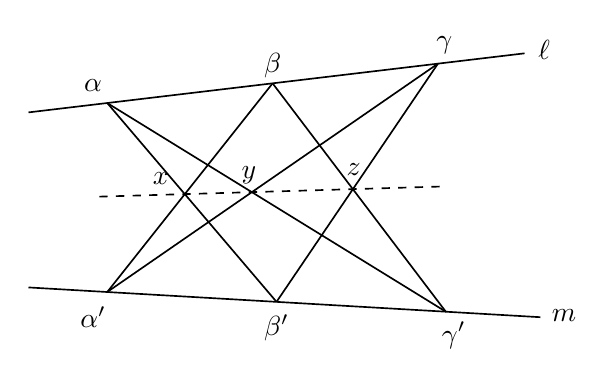
\begin{tikzpicture}[semithick]
  \draw (-1.0,2.281) -- (5.3,3.031);
  \node at (5.55,3.08) {$\ell$};
  \draw (-1.0,0.058) -- (5.5,-0.320);
  \node at (5.8,-0.30) {$m$};
  \draw (0,2.4) -- (2.15,-0.125);
  \draw (0,2.4) -- (4.3,-0.25);
  \draw (2.1,2.65) -- (0,0);
  \draw (2.1,2.65) -- (4.3,-0.25);
  \draw (4.2,2.9) -- (0,0);
  \draw (4.2,2.9) -- (2.15,-0.125);
  \draw[dashed] (-0.10,1.211) -- (4.29,1.341);
  \node at (-0.18,2.62) {$\alpha$};
  \node at (2.1,2.88) {$\beta$};
  \node at (4.28,3.13) {$\gamma$};
  \node at (-0.18,-0.32) {$\alpha'$};
  \node at (2.15,-0.45) {$\beta'$};
  \node at (4.4,-0.55) {$\gamma'$};
  \node at (0.68,1.44) {$x$};
  \node at (1.80,1.48) {$y$};
  \node at (3.13,1.56) {$z$};
\end{tikzpicture}
\caption{\trPappus{}定理。（依原书手绘图重绘。）}\label{fig:pappus}
\end{figure}

\begin{figure}[htbp]
\centering
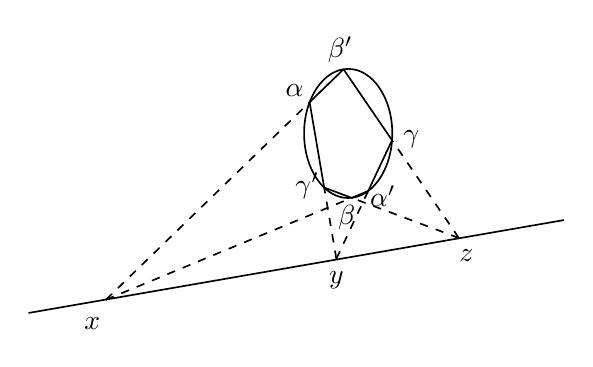
\begin{tikzpicture}[semithick]
  \draw (-4.06,-2.28) -- (2.74,-1.10);
  \draw[dashed] (-3.076,-2.111) -- (-0.490,0.397);
  \draw[dashed] (-3.076,-2.111) -- (0.044,-0.818);
  \draw[dashed] (-0.150,-1.592) -- (-0.305,-0.687);
  \draw[dashed] (-0.150,-1.592) -- (0.254,-0.731);
  \draw[dashed] (1.406,-1.328) -- (0.557,-0.086);
  \draw[dashed] (1.406,-1.328) -- (0.044,-0.818);
  \draw (0,0) ellipse (0.56 and 0.82);
  \draw (-0.490,0.397) -- (-0.305,-0.687);
  \draw (-0.305,-0.687) -- (0.044,-0.818);
  \draw (0.044,-0.818) -- (0.254,-0.731);
  \draw (0.254,-0.731) -- (0.557,-0.086);
  \draw (0.557,-0.086) -- (-0.059,0.815);
  \draw (-0.059,0.815) -- (-0.490,0.397);
  \node at (-0.10,1.06) {$\beta'$};
  \node at (-0.68,0.55) {$\alpha$};
  \node at (0.80,-0.07) {$\gamma$};
  \node at (-0.52,-0.66) {$\gamma'$};
  \node at (0.44,-0.80) {$\alpha'$};
  \node at (-0.02,-1.07) {$\beta$};
  \node at (-3.25,-2.42) {$x$};
  \node at (-0.15,-1.87) {$y$};
  \node at (1.50,-1.55) {$z$};
\end{tikzpicture}
\caption{\trPascal{}的「神秘六边形」定理。（依原书手绘图重绘。）}\label{fig:pascal}
\end{figure}

\textbf{19.4.D.（练习）}\quad 设 $\alpha$、$\beta$、$\gamma$、$\alpha'$、$\beta'$ 是 $\mathbb{P}^2_{\mathbb{R}}$ 中五个点，其中任何三点都不共线。证明：存在唯一的\trConic{} $K$ 经过这五个点。证明 $K$ 是\trRegular{}的。解释如何只用一把直尺（straightedge）构造 $K$ 在 $\alpha$ 处的\trTangentLine。（最后一部分的提示：应用\trPascal{}定理，取 $\gamma'=\alpha$。你或许需要先弄清楚，为什么在这个退化情形下还能应用\trPascal{}定理。）

特别地，给定一个椭圆 $K\subset\mathbb{R}^2$ 与一点 $\alpha\in K$，你现在将能够只用一把直尺构造 $K$ 在 $\alpha$ 处的\trTangentLine。

\textbf{19.4.5.}\ \emph{\mbox{\trPascal{}定理~19.4.4} 的证明。}\quad 我们希望证明：直线 $\overline{xy}$ 与 $\overline{\beta\gamma'}$ 及 $\overline{\beta'\gamma}$ 相交于同一个点。令 $C$ 为由 $K$ 与直线 $\overline{xy}$ 之并所成的曲线。（警告，参看 \S19.2.1：本章仅此一次，我们不假设 $C$ \trRegular！）

令 $D_1$ 为三条直线 $\overline{\alpha\beta'}$、$\overline{\beta\gamma'}$、$\overline{\gamma\alpha'}$ 之并，并令 $D_2$ 为三条直线 $\overline{\alpha'\beta}$、$\overline{\beta'\gamma}$、$\overline{\gamma'\alpha}$ 之并。注意：$D_1$ 与 $C$ 相交于九个点 $\alpha$、$\beta$、$\gamma$、$\alpha'$、$\beta'$、$\gamma'$、$x$、$y$ 以及 $\overline{xy}\cap\overline{\beta\gamma'}$，而 $D_2$ 与 $C$ 相交于同样这九个点，只是其中 $\overline{xy}\cap\overline{\beta\gamma'}$ 换成了 $\overline{xy}\cap\overline{\beta'\gamma}$。于是，倘若我们知道\mbox{推论~19.4.2} 能够适用于我们这条 $C$（它是奇异的），那么就已大功告成（参看\mbox{练习~19.4.C}）。

于是我们把\mbox{推论~19.4.2} 扩充到我们的情形。为此，我们先把\mbox{命题~19.4.1} 扩充到我们的情形。我们有一条平面三次\trCurve{} $C$，它是一条直线 $L$ 与一条\trConic{} $K$ 之并；还有两个点 $p=\overline{xy}\cap\overline{\beta\gamma'}$ 与 $q=\overline{xy}\cap\overline{\beta'\gamma}$，满足 $\OO(p)\cong\OO(q)$。（理由：二者都由 $\OO_{\mathbb{P}^2}(3)$ 限制到 $C$ 上、再经 $-(\alpha+\beta+\gamma+\alpha'+\beta'+\gamma'+x+y)$ 扭转而得。）称这个\trInvertibleSheaf{}为 $\mathscr{L}$。设 $p\ne q$。那么，$\mathscr{L}$ 的在 $p$ 与 $q$ 处取零点的两个截面给出一个\trBasePointFree\trLinearSystem，从而给出一个\trMorphism{} $\pi\colon C\to\mathbb{P}^1$，满足 $\pi^{-1}(0)=p$、$\pi^{-1}(\infty)=q$。

由\mbox{命题~19.4.1} 证明中的论证，$\pi$ 给出 $L$ 与 $\mathbb{P}^1$ 的一个同构。由于 $\pi$ 是\trProper{}的，故 $\pi(K)$ 是闭的；又由于 $K$ \trIrreducible，故 $\pi(K)$ \trIrreducible。由于 $\pi(K)$ 不包含 $0$（或 $\infty$），它不可能是整个 $\mathbb{P}^1$。于是 $\pi(K)$ 是一个点。

这条\trConic{} $K$ 与直线 $L$ 相交于两个点（计重数）——由平面曲线的\trBezout{}定理（\S18.6.4），或由简单的代数可知。若 $K\cap L$ 由两个点 $a$ 与 $b$ 组成，我们便得到矛盾：$K$ 不可能既收缩到 $\pi(a)$ 又收缩到 $\pi(b)$。但如果 $K$ 与 $L$ 相交于一点，也就是说，如果这条\trConic{}与这条直线相切，又会如何？

\textbf{19.4.E.（练习）}\quad 通过处理这个情形来完成\trPascal{}定理的证明。提示：幂零元将前来救场。直观如下：$K\cap L$ 是 $L$ 的一个\trLength{}为 $2$ 的子概形（概形的\trLength{}定义于 \S6.5.8），但可以证明，\trSchemeTheoreticImage{} $\pi(K)$ 是一个\trReduced{}闭点。

\begin{flushright}
$\square$
\end{flushright}

\textbf{19.4.6.}\ \emph{\trhRemark{}。}\quad 作为我们论证之动机的关键事实——\mbox{命题~19.4.1}——核心上是关于\trGenus{}非 $0$ 的\trCurve{}的；然而，\trPappus{}定理与\trPascal{}定理所牵涉的一切\trCurve{}却都具有\trGenus{} $0$。要记在心里的洞见是：\trGenus{} $0$ 的诸\trCurve{}之并未必具有\trGenus{} $0$。在我们的情形中，要紧的是三次\trCurve{}具有\trGenus{} $1$，哪怕它们是若干个 $\mathbb{P}^1$ 的并。


\section{\trHyperelliptic\trCurve}

接下来，我们讨论一类重要的\trCurve，即\trHyperelliptic\trCurve。在本节中，\emph{我们假设 $k$ 是\trCharacteristic{}不为 $2$ 的\trAlgClosedField}。（这些假设都可以放宽，但要付出一些代价。）

一条（射影、正则、整的）\trGenus{} $g$ \trCurve{} $C$ 称为\textbf{\trHyperelliptic}的（hyperelliptic），若它容许一个 $\mathbb{P}^1_k$ 的\trDoubleCover（即一个到 $\mathbb{P}^1_k$ 的、次数为 $2$ 的、必然有限的\trMorphism）。（关于从\trCurve{}到\trCurve{}的映射的次数的讨论，见 \S16.3.4。）为方便起见，当我们说 $C$ 是\trHyperelliptic{}的时，我们心目中便隐含着一个\trDoubleCover $\pi\colon C\to\mathbb{P}^1$ 的\emph{选取}。（我们日后会看到，若 $g\ge 2$，则这样的\trDoubleCover{}至多只有一个，见\mbox{命题~19.5.7}，所以这并不是一个多大的假设。）映射 $\pi$ 称为\textbf{\trHyperelliptic{}映射}（hyperelliptic map）。

由\mbox{练习~16.3.D}，$\mathbb{P}^1$ 的任一\trClosedPoint{} $p$ 的原像要么由一个点组成，要么由两个点组成。若 $\pi^{-1}(p)$ 是单个点，我们就说 $p$ 是一个\textbf{\trBranchPoint}（branch point），而 $\pi^{-1}(p)$ 是 $\pi$ 的一个\textbf{\trRamification{}点}（ramification point）。（\trRamification{}这一概念将在 \S21.7 中以更一般的方式定义。）

\textbf{19.5.1.\ \trhTheorem（\trHyperelliptic{}\trRiemann--\trHurwitz{}公式）。}\ ——\ \emph{设 $k=\bar{k}$ 且 $\operatorname{char}k\ne 2$，而 $\pi\colon C\to\mathbb{P}^1_k$ 是由 $k$ 上一条射影、正则、不可约、\trGenus{}为 $g$ 的\trCurve{}给出的\trDoubleCover。则 $\pi$ 有 $2g+2$ 个\trBranchPoint。}

这是\trRiemann--\trHurwitz{}公式的一个特例；我们将在 \S21.4 中陈述并证明该公式。你或许早已听说过：\trGenus{} $1$ 的复曲线会\trDoubleCover $\mathbb{P}^1$，并且在四个点上\trRamification。

为了证明\mbox{定理~19.5.1}，我们先证明下面这条。

\textbf{19.5.2.\ \trhProposition。}\ ——\ \emph{设 $\operatorname{char}k\ne 2$ 且 $k=\bar{k}$。给定 $\mathbb{P}^1$ 中 $r$ 个互不相同的点 $p_1,\dots,p_r$，则当 $r$ 为偶数时，恰有一个\trDoubleCover{}恰在这些点处\trRamification；而当 $r$ 为奇数时，则一个也没有。}

\emph{证明。}\quad 在 $\mathbb{P}^1$ 中取两点 $0$ 与 $\infty$，它们都不同于这 $r$ 个\trBranchPoint。全部\trBranchPoint{}都落在 $\mathbb{P}^1-\infty=\mathbb{A}^1=\Spec k[x]$ 之中。假设我们有 $\mathbb{A}^1$ 的一个\trDoubleCover $C'\to\mathbb{A}^1$，其中 $x$ 是 $\mathbb{A}^1$ 上的\trCoordinate。这便诱导出一个 $k(x)$ 上的二次\trFieldExtension{} $K$。由于 $\operatorname{char}k\ne 2$，这个扩张是\trGalois{}的。令 $\sigma\colon K\to K$ 为那个\trGalois{}\trInvolution。取 $K$ 中一个满足 $\sigma(y)=-y$ 的非零元素 $y$，于是 $1$ 与 $y$ 构成 $K$ 在域 $k(x)$ 上的一组基，并且二者都是 $\sigma$ 的特征向量。现在 $\sigma(y^2)=y^2$，故 $y^2\in k(x)$。我们可以用 $y$ 的一个适当的 $k(x)$ 倍替代 $y$，使得 $y^2$ 是一个无重因式的首一多项式。（我们正是在这里用到了 $k$ \trAlgClosed{}这一假设，为的是得到首项系数 $1$。）

于是 $y^2=x^N+a_{N-1}x^{N-1}+\cdots+a_0$，其中右边的多项式（记作 $f(x)$）无重根。正则性的\trJacobianCriterion（以\mbox{练习~13.2.F} 的面目出现）蕴涵：$\mathbb{A}^2=\Spec k[x,y]$ 中的这条\trCurve{} $C'_0$ 是\trRegular{}的。于是 $C'_0$ 是\trNormal{}的，并且与 $C'$ 具有相同的\trFunctionField。从而 $C'_0$ 与 $C'$ 都是 $\mathbb{A}^1$ 在由 $y$ 生成的那个域的有限扩张中的正规化，故二者\trIsomorphic。这样，我们便以一个显式的方程认出了 $C'$。

\trBranchPoint{}对应于那些使得 $y$ 恰有一个值的 $x$ 值，也就是说，对应于 $f(x)$ 的根。特别地，$N=r$，且
\[
f(x)=(x-p_1)\cdots(x-p_r),
\]
其中诸 $p_i$ 被理解为 $\bar{k}$ 中的元素。

在掌握了 $\mathbb{A}^1$ 上的情形之后，我们回到 $\mathbb{P}^1$ 上的情形。我们将考察这个\trBranchedCover{}在仿射开集 $\mathbb{P}^1\setminus\{0\}=\Spec k[u]$ 上的情形，其中 $u=1/x$。把上面的论证施加于 $\Spec k[u]$ 而非 $\Spec k[x]$，便表明任何这样的\trDoubleCover{}都必形如
\[
\begin{aligned}
C''&=\Spec k[Z,u]\big/\bigl(Z^2-(u-1/p_1)\cdots(u-1/p_r)\bigr)\\
&=\Spec k[Z,u]\Big/\Bigl(\bigl((-1)^r\textstyle\prod p_i\bigr)Z^2-u^rf(1/u)\Bigr)\\
&\longrightarrow \Spec k[u]=\mathbb{A}^1.
\end{aligned}
\]
因此，若在整个 $\mathbb{P}^1$ 上存在一个\trDoubleCover，则它必定是把 $C''$ 粘合到 $C'$ 上而得到的——这次粘合架在 $\Spec k[x]$ 与 $\Spec k[u]$ 粘合成 $\mathbb{P}^1$ 的那次粘合「之上」。

于是在 $K(C)$ 中，必有
\[
z^2=u^rf(1/u)=f(x)/x^r=y^2/x^r
\]
（其中 $z$ 是用 $(-1)^r\prod p_i$ 的一个平方根去乘 $Z$ 而得到的），由此 $z^2=y^2/x^r$。

若 $r$ 为偶数，把 $K(C)$ 看作由 $y$ 与 $x$ 生成的，则 $z$ 有两个可能的值：$z=\pm y/x^{r/2}$。必要时把 $z$ 改名为 $-z$ 之后，把这两块粘起来的方式便只有一种（我们取正的那个平方根）。

若 $r$ 为奇数，则结论由下面的\mbox{练习~19.5.A} 得出。

\textbf{19.5.A.（练习）}\quad 设 $\operatorname{char}k\ne 2$。证明：$x$ 在域 $k(x)[y]/(y^2-f(x))$ 中没有平方根，其中 $f$ 是一个根 $p_1,\dots,p_r$ 皆非零的多项式。（一个可能的提示：为什么 $\sqrt{3}\notin\mathbb{Q}(\sqrt{2})$？）请解释这如何证明 $r$ 为奇数时的\mbox{命题~19.5.2}。

\begin{flushright}
$\square$
\end{flushright}

为日后参考计，我们在此把\trHyperelliptic{}覆盖 $C\to\mathbb{P}^1$ 的这个显式的（双仿射）描述汇总如下。
\begin{equation*}\tag{19.5.2.1}\label{eq:hyperelliptic-two-affine}
\begin{tikzcd}[row sep=3.2em]
\Spec k[x,y]/(y^2-f(x)) \dar \rar["z=y/x^{r/2}","y=z/u^{r/2}"'] & \Spec k[u,z]/(z^2-u^rf(1/u)) \dar \\
\Spec k[x] \rar["u=1/x","x=1/u"'] & \Spec k[u]
\end{tikzcd}
\end{equation*}

\textbf{19.5.3.}\ \emph{若 $k$ 不\trAlgClosed。}\quad 若 $k$ 不\trAlgClosed{}（但\trCharacteristic{}不为 $2$），则上面的论证表明：若我们有 $\mathbb{A}^1$ 的一个\trDoubleCover，则它必形如 $y^2=af(x)$，其中 $f$ 是首一的（且 $a\ne 0$）。此外，若 $a$ 与 $a'$ 相差（在乘法意义下）一个 $(k^\times)^2$ 中的元素，则 $y^2=af(x)$ \trIsomorphic{}于 $y^2=a'f(x)$。你或许能利用这一点证明：（在 $k^\times\ne(k^\times)^2$ 的假设下）\trDoubleCover\emph{并不}由其\trBranchPoint{}决定。而且，这一失效由 $k^\times/(k^\times)^2$ 所分类。于是，我们有大量的\trCurve，它们在 $k$ 上互不\trIsomorphic，但在 $\bar{k}$ 上却变得\trIsomorphic。它们常被称作彼此的\emph{扭曲}（twists）。

（特别地，一旦我们定义了\trEllipticCurve，你将能够证明：$\mathbb{Q}$ 上存在两条具有相同的 $j$-不变量却互不\trIsomorphic{}的\trEllipticCurve；见\mbox{练习~19.10.H}。）

\textbf{19.5.4.}\ \emph{回到\trHyperelliptic{}\trRiemann--\trHurwitz{}公式（\mbox{定理~19.5.1}）的证明。}\quad 我们对 $\mathbb{P}^1$ 的那个在 $r$ 个不同点处\trRamification{}的唯一\trDoubleCover{}的显式描述，将使我们得以算出\trGenus，从而完成\mbox{定理~19.5.1} 的证明。

我们沿用\mbox{命题~19.5.2} 之证明中的记号 \eqref{eq:hyperelliptic-two-affine}。设 $\mathbb{P}^1$ 照例由 $\Spec k[x]$ 与 $\Spec k[u]$ 组成仿射覆盖，其中 $u=1/x$。设 $C\to\mathbb{P}^1$ 是一个\trDoubleCover，在 $\Spec k[x]$ 上由 $y^2=f(x)$ 给出，其中 $f$ 的次数为 $r$，且 $z^2=u^rf(1/u)$。那么 $C$ 有一个由 $\Spec k[x,y]/(y^2-f(x))$ 与 $\Spec k[u,z]/(z^2-u^rf(1/u))$ 组成的仿射开覆盖。$\OO_C$ 相应的\trCech\trComplexN{}为
\[
\begin{aligned}
0\longrightarrow k[x,y]/(y^2-f(x))\times k[u,z]/(z^2-u^rf(1/u))\overset{d}{\longrightarrow}{}\\
(k[x,y]/(y^2-f(x)))_x\longrightarrow 0.
\end{aligned}
\]
复形的第二个（也是最后一个）非零部分有一组由单项式 $x^ny^\epsilon$ 构成的基，其中 $n\in\mathbb{Z}$，而 $\epsilon=0$ 或 $1$。为计算\trGenus{} $g=h^1(C,\OO_C)$，我们必须计算 $\coker d$。我们可以用第一个因子 $k[x,y]/(y^2-f(x))$ 打到单项式 $x^ny^\epsilon$，其中 $n\in\mathbb{Z}^{\ge 0}$，而 $\epsilon=0$ 或 $1$。第二个因子的像由形如 $u^mz^\epsilon$ 的元素生成，其中 $m\ge 0$，而 $\epsilon=0$ 或 $1$。但 $u^mz^\epsilon=x^{-m}(y/x^{r/2})^\epsilon$。检视即知，余核有一组由单项式 $x^{-1}y$、$x^{-2}y$、……、$x^{-r/2+1}y$ 生成的基，从而其维数为 $r/2-1$。于是 $g=r/2-1$，\mbox{定理~19.5.1} 随之得证。

\begin{flushright}
$\square$
\end{flushright}

\textbf{19.5.5.}\ \emph{各种\trGenus{}的\trCurve。}\quad 作为\trHyperelliptic{}\trRiemann--\trHurwitz{}公式（\mbox{定理~19.5.1}）的一个推论，我们看到：在\trCharacteristic{}不为 $2$ 的\trAlgClosedField{}上，每个\trGenus{} $g\ge 0$ 都有\trCurve：要得到一条\trGenus{}为 $g$ 的\trCurve，只需考虑在 $2g+2$ 个互不相同的点处\trRamification{}的那个\trBranchedCover。唯一的那条\trGenus{} $0$ \trCurve{}就属于这种形式；我们将在 \S19.6.2 中看到，每条\trGenus{} $2$ 的\trCurve{}也都属于这种形式。我们马上就会看到，每条\trGenus{} $1$ 的\trCurve{}（提醒：在\trAlgClosedField{}上！）也是如此（\S19.9.5）。但指望一切\trCurve{}都属于这种形式就想得太多了；我们马上就会看到（\S19.7.4），存在\emph{不}是\trHyperelliptic{}的\trGenus{} $3$ \trCurve，而且我们甚至会得到「大多数」\trGenus{} $3$ \trCurve{}都不是\trHyperelliptic{}的这番启发式证据。日后我们还会给出（可以使之精确化的）模糊证据，表明当 $g>2$ 时「大多数」\trGenus{} $g$ \trCurve{}都不是\trHyperelliptic{}的（\S19.8.4）。

\textbf{19.5.B.（练习）}\quad 验证：一条\trGenus{}至少为 $1$ 的\trCurve{} $C$ 容许一个到 $\mathbb{P}^1$ 的次数 $2$ 覆盖，当且仅当它容许一个满足 $h^0(C,\mathscr{L})=2$ 的次数 $2$ \trInvertibleSheaf{} $\mathscr{L}$。在做这件事的过程中，你可能还愿意顺带验证：若 $C$ 是一条\trGenus{}至少为 $1$ 的\trCurve，而 $C$ 有一个带有至少 $2$ 个（线性无关的）截面的次数 $2$ \trInvertibleSheaf{} $\mathscr{L}$，则 $\mathscr{L}$ 恰有两个截面，并且这个 $\mathscr{L}$ 是\trBasePointFree{}的，从而给出一个\trHyperelliptic{}映射。

\textbf{19.5.6.\ \trhProposition。}\ ——\ \emph{设 $g\ge 2$。若 $\mathscr{L}$ 对应于一个\trHyperelliptic{}覆盖 $C\to\mathbb{P}^1$，则 $\mathscr{L}^{\otimes(g-1)}\cong\omega_C$。}

\emph{证明。}\quad 把\trHyperelliptic{}映射与第 $g-1$ 个\trVeroneseEmbedding{}复合：
\begin{equation*}\tag{19.5.6.1}\label{eq:hyperelliptic-veronese}
\begin{tikzcd}
C \rar["|\mathscr{L}|"] & \mathbb{P}^1 \rar["\nu_{g-1}\cong|\OO_{\mathbb{P}^1}(g-1)|"] & \mathbb{P}^{g-1}.
\end{tikzcd}
\end{equation*}
该复合对应于 $\mathscr{L}^{\otimes(g-1)}$。这个\trInvertibleSheaf{}的\trDegree{}为 $2g-2$（由\mbox{练习~18.4.G}）。

接下来我们证明拉回映射 $\mathrm{H}^0(\mathbb{P}^{g-1},\OO(1))\to\mathrm{H}^0(C,\mathscr{L}^{\otimes(g-1)})$ 是单射；也就是说，任一非零的 $s\in\mathrm{H}^0(\mathbb{P}^{g-1},\OO(1))$ 都拉回成 $\mathrm{H}^0(C,\mathscr{L}^{\otimes(g-1)})$ 中的一个非零元素；换言之，$C$ 在 $\mathbb{P}^{g-1}$ 中的像是非退化的。这是因为 $C$ 在 $\mathbb{P}^{g-1}$ 中的像正是 $\mathbb{P}^1$ 经 $\nu_{g-1}$ 的像（一条\trRationalNormalCurve；见 \S9.3.6）；而 $\mathbb{P}^1$ 在完全线性系 $|\OO_{\mathbb{P}^1}(g-1)|$ 之下的像是非退化的（\mbox{练习~15.2.C}）。

于是 $\mathscr{L}^{\otimes(g-1)}$ 至少有 $g$ 个截面。但由\mbox{练习~19.2.A}，\trDegree{}为 $2g-2$ 且带有（至少）$g$ 个截面的\trInvertibleSheaf{}只有\trCanonical{}层。

\begin{flushright}
$\square$
\end{flushright}

作为额外附赠，我们看到 \eqref{eq:hyperelliptic-veronese} 的复合正是\emph{完全}线性系 $|\mathscr{L}^{\otimes(g-1)}|$——$\mathscr{L}^{\otimes(g-1)}$ 的一切截面都由此而来。

\textbf{19.5.7.\ \trhProposition（\trGenus{} $\ge 2$ 的\trCurve{}至多以一种方式成为\trHyperelliptic）。}\ ——\ \emph{任何一条\trGenus{}至少为 $2$ 的\trCurve{} $C$ 都至多容许 $\mathbb{P}^1$ 的一个\trDoubleCover。更精确地说，若 $\mathscr{L}$ 与 $\mathscr{M}$ 是给出映射 $C\to\mathbb{P}^1$ 的两个次数 $2$ 的\trLineBundle，则 $\mathscr{L}\cong\mathscr{M}$。}

\emph{证明。}\quad 若 $C$ 是\trHyperelliptic{}的，则我们可以通过考虑由 $\omega_C$ 给出的\trCanonical\trLinearSystem{}找回那个\trHyperelliptic{}映射（即\textbf{\trCanonical{}映射}（canonical map），我们在接下来的几节中还要反复用到它）：它是到一个\trDegree{}为 $g-1$ 的\trRationalNormalCurve{}的\trDoubleCover（由前一条\trhProposition），而那条有理正规曲线\trIsomorphic{}于 $\mathbb{P}^1$。这个\trDoubleCover{}就是那个\trHyperelliptic{}覆盖（这同样由前一条\trhProposition{}的证明可知）。于是，\trHyperelliptic{}覆盖 $C\to\mathbb{P}^1$ 由\trCanonical{}映射所决定（故至多只有一个）。这个映射 $C\to\mathbb{P}^1$ 必须同时由 $\mathscr{L}$ 与 $\mathscr{M}$ 诱导，从而 $\mathscr{L}\cong\mathscr{M}$（利用把到\trProjectiveSpace{}的映射与\trLineBundle{}联系起来的\mbox{定理~15.2.2}）。

\begin{flushright}
$\square$
\end{flushright}

\textbf{19.5.C.（练习）}\quad 设 $C$ 是一条\trGenus{}至少为 $2$ 的\trHyperelliptic\trCurve。证明：\trHyperelliptic{}\trInvolution{}与 $C$ 的任何其他\trAutomorphism{} $g$ 交换。（提示：当你用 $g$ 去共轭这个\trInvolution{}时，会发生什么？）

\textbf{19.5.8.}\ \emph{「\trHyperelliptic\trCurve{}的空间」。}\quad 多亏了\mbox{命题~19.5.7}，我们现在可以分类\trGenus{}至少为 $2$ 的\trHyperelliptic\trCurve{}了。\trGenus{} $g\ge 2$ 的\trHyperelliptic\trCurve{}恰好对应于 $\mathbb{P}^1$ 上的 $2g+2$ 个互不相同的点——模掉 $S_{2g+2}$，也模掉 $\mathbb{P}^1$ 的\trAutomorphism。于是，「\trHyperelliptic\trCurve{}的空间」的维数为
\[
2g+2-\dim\Aut\mathbb{P}^1=2g-1.
\]
这并不是一个良定义的陈述，因为我们尚未严格地定义「\trHyperelliptic\trCurve{}的空间」——它是一个\trModuliSpace{}的一个例子。眼下，且把这当作一条合情合理的陈述。这个空间不可约且既约，这一点同样合情——它是某个不可约且既约之物的像。


\section{\trGenus{} $2$ 的\trCurve}

\textbf{19.6.1. 把\trGenus{} $1$ 留待日后的缘由。}\quad 此刻就直接跳到\trGenus{} $1$，或许是最顺理成章的做法，但\trEllipticCurve{}的理论格外丰富而精微，所以我们把它留到 \S19.9。

一般来说，视 $g=0$、$g=1$ 还是 $g\ge 2$ 而定，\trCurve{}会呈现出颇为不同的性态（拓扑地、算术地、几何地）。这种三分法可以延伸到更高维的\trVariety。在\trCurve{}的情形，我们对此已有了一些初步的体会。算术上，\trGenus{} $0$ 的\trCurve{}可以有许多许多\trRationalPoint，\trGenus{} $1$ 的\trCurve{}可以有许多\trRationalPoint，而由\trFaltings{}定理（\trMordell{}猜想），\trGenus{}至少为 $2$ 的任何\trCurve{}都至多只有有限多个\trRationalPoint。（于是，早在\trTaniyama--\trShimura{}猜想 [Wi, TWi] 的若干重要情形——从而\trFermat{}大定理——得到证明之前，我们就已经知道：$\mathbb{P}^2$ 中的 $x^n+y^n=z^n$ 在 $n\ge 4$ 时至多只有有限多个有理解，因为这类\trCurve{}的\trGenus{}为 $\binom{n-1}{2}>1$；见 \eqref{eq:genus-plane-curve}。）用微分几何的语言来说：\trGenus{} $0$ 的\trRiemannSurface{}具有正曲率，\trGenus{} $1$ 的\trRiemannSurface{}是平坦的，而\trGenus{}至少为 $2$ 的\trRiemannSurface{}具有负曲率。事实是：\trGenus{}至少为 $2$ 的\trCurve{}具有有限的\trAutomorphismGroup（见 \S21.4.9），而\trGenus{} $1$ 的\trCurve{}具有一维的\trAutomorphismGroup（见\mbox{问题~19.10.6}），并且\trAlgClosedField{}上唯一的那条\trGenus{} $0$ \trCurve{}具有三维的\trAutomorphismGroup（见\mbox{练习~15.5.A} 与\mbox{练习~15.5.B}）。（关于这一话题的更多内容，见\mbox{练习~21.5.F}。）

\textbf{19.6.2. 回到\trGenus{} $2$ 的\trCurve。}

在\trAlgClosedField{}上，我们在 \S19.3 中看到：\trGenus{} $0$ 的\trCurve{}只有一条。在 \S19.5 中，我们确立了：存在\trGenus{} $2$ 的超椭圆\trCurve。可我们要怎样才能把\trGenus{} $2$ 的\trCurve{}真正拿到手呢？例如，它们全都超椭圆吗？它们有「多少」条？我们现在就来着手处理这些问题。

取定一条\trGenus{}为 $g=2$ 的\trCurve{} $C$。此时 $\omega_C$ 的\trDegree{}为 $2g-2=2$，并且带有两个截面（\mbox{练习~19.2.A}）。由\mbox{练习~19.5.B}，$\omega_C$ 是\trBasePointFree{}的，从而诱导出一个二重覆盖 $C\to\mathbb{P}^1$（在 $\mathbb{P}^1$ 的\trAutomorphism{}之下唯一；这些\trAutomorphism{}我们在 \S15.5.2 中研究过）。反过来，任何一个二重覆盖 $C\to\mathbb{P}^1$ 都来自一个带有至少两个截面的、次数为 $2$ 的\trInvertibleSheaf。于是，若 $g(C)=2$，这个\trInvertibleSheaf{}就必定是\trCanonical{}层——理由无他：它是一个\trDegree{}为 $2g-2=2$、带有 $g=2$ 个截面的\trLineBundle（或者，换个思路，由\mbox{命题~19.5.6} 的最容易情形也可得出）。

于是，在\trGenus{} $2$ 的\trCurve{}与 $\mathbb{P}^1$ 的\trGenus{} $2$ 二重覆盖（在 $\mathbb{P}^1$ 的\trAutomorphism{}意义下）之间，我们便有了一个自然的\trBijection。若\trCharacteristic{}不为 $2$，则超椭圆\trRiemann--\trHurwitz{}公式（\mbox{定理~19.5.1}）表明：这个二重覆盖在 $2g+2=6$ 个几何点上分歧。特别地，我们有一「个三维的\trGenus{} $2$ \trCurve{}空间」。这并不严格，但我们当然能够证明：存在无穷多条\trGenus{} $2$ 的\trCurve。确切地说：

\textbf{19.6.A.（练习）}\quad 取定一个\trCharacteristic{}不为 $2$ 的\trAlgClosedField{} $k$。证明：$k$ 上存在无穷多条（两两）互不\trIsomorphic{}的\trGenus{} $2$ \trCurve。

\textbf{19.6.B.（练习）}\quad 证明：每条\trGenus{} $2$ 的\trCurve{}（在\trCharacteristic{}不为 $2$ 的任意域上）都具有有限的\trAutomorphismGroup。


\section{\trGenus{} $3$ 的\trCurve}

\textbf{19.7.1. \trCanonical{}嵌入。}

我们先就\trGenus{} $g>1$ 作一些一般性的讨论，然后再专门讨论\trGenus{} $3$。

\textbf{19.7.A.（重要练习）}\quad 设 $k=\bar{k}$（纯粹是为了避免分心——你尽可以去掉这条假设）。设 $C$ 是一条\trGenus{}为 $g$ 的\trCurve，而 $g>1$。证明：若 $C$ 不是超椭圆的，则\trCanonical{}\trInvertibleSheaf{}给出一个\trClosedEmbedding{} $C\hookrightarrow\mathbb{P}^{g-1}$。（在超椭圆的情形，我们已经见过：\trCanonical{}层给出的是到一个\trRationalNormalCurve{}的二重覆盖。）提示：回想 $h^0(C,\omega_C)=g$（\mbox{练习~19.2.A}）。使用我们在 \S19.1 中的那个「闭嵌入判别法」，即以其 \S19.2.10 的形式。回想：若 $h^0(C,\OO(p+q))=2$，则 $C$ 是超椭圆的（\mbox{练习~19.5.B}）。

这道练习给出了「一切\trGenus{} $2$ \trCurve{}都是超椭圆的」的第二个证明。

\textbf{19.7.2.}\ \emph{\trhDefinition{}。}\quad 这样一条经\trCanonical{}层（又称\trCanonical{}\trLineBundle）嵌入 $\mathbb{P}^{g-1}$ 的\trCurve{}称为\textbf{\trCanonical{}曲线}（canonical curve），而这个\trClosedEmbedding{}则称为 $C$ 的\textbf{\trCanonical{}嵌入}（canonical embedding）。

\textbf{19.7.3. 回到\trGenus{} $3$。}

现在设 $C$ 是一条\trGenus{} $3$ 的\trCurve。那么 $\omega_C$ 的\trDegree{}为 $2g-2=4$，并且带有 $g=3$ 个\trSection。由\mbox{练习~19.7.A}，当（且仅当）$C$ 不是超椭圆的时，\trCanonical{}映射便把 $C$ 描述为 $\mathbb{P}^2$ 中一条\trDegree{}为 $4$ 的\trCurve。

反过来，任何\trPlaneQuartic{}都是被典范地嵌入的。理由：这条\trCurve{}具有\trGenus{} $3$（见 \eqref{eq:genus-plane-curve}），并且由一个\trDegree{}为 $4$、带有三个\trSection{}的\trInvertibleSheaf{}所映射。但由\mbox{练习~19.2.A}，\trDegree{}为 $2g-2$ 且带有 $g$ 个\trSection{}的\trInvertibleSheaf{}只有 $\omega_C$。

特别地，每条非超椭圆的\trGenus{} $3$ \trCurve{}都可以恰好以一种方式描述为\trPlaneQuartic{}（在 $\mathbb{P}^2$ 的\trAutomorphism{}之下；这些\trAutomorphism{}已在\mbox{练习~15.5.A} 中得到描述）。我们已然证明：在模掉\trProjectiveTransformation{}（\S15.5.2）的意义下，非超椭圆的\trGenus{} $3$ \trCurve{}与\trPlaneQuartic{}之间存在一个\trBijection。

\textbf{19.7.4.}\ \emph{\trhRemark{}。}\quad 特别地，由于存在\trRegular{}的\trPlaneQuartic（\mbox{练习~13.3.E}），故存在非超椭圆的\trGenus{} $3$ \trCurve。

\textbf{19.7.B.（练习，参看 \S19.5.8）}\quad 给出一个启发式（非严格）的论证：非超椭圆的\trGenus{} $3$ \trCurve{}构成一个维数为 $6$ 的族。（提示：数一数\trRegular{}\trPlaneQuartic{}之族的维数，再模掉 $\Aut\mathbb{P}^2=\mathrm{PGL}(3)$。）

于是，\trGenus{} $3$ 的\trCurve{}看似分属两个族：超椭圆\trCurve{}（一个维数为 $5$ 的族）与非超椭圆\trCurve{}（一个维数为 $6$ 的族）。这是一种假象——它们实际上同属一个维数为 $6$ 的族。事实上，超椭圆\trCurve{}自然地就是非超椭圆\trCurve{}的极限。我们可以写下一个显式的族。（这番解释不可避免地需要一些「挥手而过」的成分\footnote{译注：原文 \emph{hand-waving}，指不作严格证明、以手势示意带过的论证方式。}，因为它牵涉到我们尚未见过的论题。）设我们有一条在 $\mathbb{P}^1$ 的 $2g+2=8$ 个点处分支的超椭圆\trCurve。选取一个把 $\mathbb{P}^1$ 与 $\mathbb{P}^2$ 中一条\trConic{}等同起来的\trIsomorphism。于是存在一条\trRegular{}的\trPlaneQuartic，恰好在那八个点处与这条\trConic{}相交。（这需要一个用到\trBertini{}定理~\mbox{13.4.2} 的简短论证，我们略去。）于是，若 $f$ 是这条\trConic{}的方程，而 $g$ 是这条四次曲线的方程，则 $f^2+t^2g$ 便是一族对大多数 $t$ 都\trSmooth{}的四次曲线（光滑性是 $t$ 的一个开条件，见关于一般光滑性的\mbox{定理~21.6.6}）。$t=0$ 的情形是一条二重\trConic。而事实是：若你把这个族的\trTotalSpace{}\trNormalization，则中心纤维（在 $t=0$ 之上者）就变成了我们的超椭圆\trCurve。这样，我们便把这条超椭圆\trCurve{}表示成了非超椭圆\trCurve{}的极限。

\textbf{19.7.C.（不重要练习）}\quad 把容许一个到 $\mathbb{P}^1$ 的\trDegree{} $3$ 覆盖的（射影）\trCurve{}（在域 $k$ 上）称为\textbf{\trTrigonal{}的}（trigonal）。证明：每条非超椭圆的\trGenus{} $3$ 复\trCurve{}都是\trTrigonal{}的：取其在 $\mathbb{P}^2$ 中的四次模型，并从曲线上任意一点向 $\mathbb{P}^1$ 作\trProjection。具体做法：在 $\mathbb{P}^2$ 上选取\trCoordinate{}，使得 $p$ 落在 $[0,0,1]$ 处。（同样的想法——施于三次曲线而非四次曲线——将在 \S19.9.9 中得到使用。）

\textbf{19.7.5.}\ \hard\ \textbf{一条没有非平凡\trAutomorphism{}的\trGenus{} $3$ \trCurve。}

我们已经看到：\trGenus{}至多为 $2$ 的（\trSmooth、\trProjective、\trIntegral{}的）\trCurve{}总有非平凡\trAutomorphism。而事实表明，存在没有非平凡\trAutomorphism{}的\trGenus{} $3$ \trCurve。

\textbf{19.7.D.（练习）}\quad 设 $C'\subset\mathbb{P}^2$ 是一条\trSmooth{}的\trPlaneQuartic{}（在任意域 $k$ 上）。证明：$C'$ 的\trAutomorphism{}与保持 $C'$ 的 $\mathbb{P}^2$ 的\trAutomorphism{}之间存在\trBijection\footnote{原书此处作「there is bijection between」，当脱一「a」，径补。——译者注}。

于是，要找一条没有非平凡\trAutomorphism{}的\trGenus{} $3$ \trCurve，我们只须找到一条\trSmooth{}的\trPlaneQuartic{} $C'$，使得 $\mathbb{P}^2$ 中把 $C'$ 作为集合予以保持的\trAutomorphism{}必为恒等映射。你的直觉或许会（正确地）告诉你：大多数四次曲线都具有这条性质。但要具体展示一个 $C'$（连同证明），就得挽起袖子真刀真枪地干了。\trPoonen{}在 [P1] 中给出了在任意域上都没有非平凡\trAutomorphism{}的\trCurve；一个特征 $0$ 的例子是
\[
y^3z-3yz^3=3x^4-4x^3z+z^4.
\]

\textbf{19.7.E.（练习）}\quad 设 $C$ 是一条没有非平凡\trAutomorphism{}的\trSmooth、\trProjective{}的\trCurve。证明：$C$ 的任何两个互不相同的\trOpenSubset{}都互不\trIsomorphic。

\textbf{19.7.6.}\ \emph{具有非平凡\trAutomorphism{}的\trGenus{} $3$ \trCurve。}

当然，\trGenus{} $3$ 的\trCurve{}可以有非平凡\trAutomorphism：超椭圆\trCurve{}便是明证。更令人赞叹的是\trKlein{}四次曲线
\[
x^3y+y^3z+z^3x=0
\]
（在 $\mathbb{P}^2_{\mathbb{C}}$ 中），它具有 $168$ 个\trAutomorphism。（你能把它们全都找出来吗？）事实上，\trKlein{}四次曲线的\trAutomorphismGroup{}是阶为 $168$ 的那个唯一的有限单群（即第二小的非阿贝尔有限单群）。在 \S21.4.9 中，我们将看到任何\trGenus{} $3$ \trCurve{}都不可能具有更多的\trAutomorphism（此处假定「\trGenus{}大于 $1$ 的\trCurve{}具有有限\trAutomorphismGroup」这一艰深的事实）。


\section{\trGenus{} $4$ 与 $5$ 的\trCurve}

我们先考虑\trGenus{} $4$ 的非超椭圆\trCurve{}$C$。注意 $\deg\omega_C=6$ 且 $h^0(C,\omega_C)=4$，所以\trCanonical{}映射把 $C$ 表为 $\mathbb{P}^3$ 中的一条六次曲线。设 $\iota\colon C\hookrightarrow\mathbb{P}^3$ 为\trCanonical{}（闭）嵌入。我们将会看到：所有这类 $C$ 都是\trQuadricSurface{}与三次曲面的\trCompleteIntersection；反之，二次曲面与三次曲面的一切\trRegular{}\trCompleteIntersection{}都是\trGenus{} $4$ 的非超椭圆\trCurve，且以\trCanonical{}方式嵌入。

由 \eqref{eq:h0-high-degree}（\trRiemannRoch{}与\trSerreDuality），
\[
h^0(C,\iota^*\OO_{\mathbb{P}^3}(2))=h^0(C,\omega_C^{\otimes 2})=\deg\omega_C^{\otimes 2}-g+1=12-4+1=9.
\]
另一方面，$h^0(\mathbb{P}^3,\OO_{\mathbb{P}^3}(2))=\binom{3+2}{2}=10$（\mbox{练习~15.1.C}）。于是\trRestrictionMap
\[
\mathrm{H}^0(\mathbb{P}^3,\OO_{\mathbb{P}^3}(2))\longrightarrow \mathrm{H}^0(C,\iota^*\OO_{\mathbb{P}^3}(2))
\]
必有非平凡\trKernel，故 $\mathbb{P}^3$ 中至少存在一张包含我们\trCurve{}$C$ 的\trQuadricSurface{} $Q$。\trQuadricSurface{}要么是\trDoublePlane，要么是两个平面之并，要么是锥，要么是\trRegular{}\trQuadricSurface。（它们分别对应\trRank{}为 $1$、$2$、$3$、$4$ 的\trQuadraticForm{}；\trQuadraticForm{}之\trRank{}的定义见\mbox{练习~5.4.J}。）但 $C$ 不可能落在一张平面内，所以 $Q$ 必是锥或\trRegular{}\trQuadricSurface。特别地，$Q$ \trIrreducible。

现在，$C$ 不可能落在两张（互不相同的）此类二次曲面上，设为 $Q$ 与 $Q'$。否则，由于 $Q$ 与 $Q'$ 没有公共\trIrreducibleComponent（它们\trIrreducible{}且互不相同！），$Q\cap Q'$ 是一条\trCurve（不必\trReduced{}或\trIrreducible）。由\trBezout{}定理（\mbox{练习~18.6.J}），$Q\cap Q'$ 是一条\trDegree{}为 $4$ 的\trCurve。于是我们的\trCurve{}$C$ 既然\trDegree{}为 $6$，就不可能包含在 $Q\cap Q'$ 之中。（若你不能直接看出这一点，\mbox{练习~18.6.E} 或许有帮助。）

\textbf{19.8.1.}\quad 接下来我们考虑三次曲面。再由 \eqref{eq:h0-high-degree}，
\[
h^0(C,\omega_C^{\otimes 3})=\deg\omega_C^{\otimes 3}-g+1=18-4+1=15.
\]
而 $\Sym^3\Gamma(C,\omega_C)$ 的维数为 $\binom{3+3}{3}=20$。于是 $C$ 至少落在一个五维的三次形式向量空间之中。其中四维的子空间来自用一个线性形式 $(?w+?x+?y+?z)$\footnote{译注：原书以问号表示未定系数。}去乘\trQuadraticForm{} $Q$。故仍剩下一个三次曲面 $K$，其底层形式不被\trQuadraticForm{} $Q$ 整除\footnote{原书此处作「quadric form」，疑当为「quadratic form」之误，兹照录原书。——译者注}（即 $K$ 不包含 $Q$）。于是 $K$ 与 $Q$ 无公共\trIrreducibleComponent，故 $K\cap Q$ 是一个包含 $C$ 作为\trClosedSubscheme{}的\trCompleteIntersection。$K\cap Q$ 与 $C$ 的\trDegree{}都是 $6$（前者由\trBezout{}定理，\mbox{练习~18.6.J}；后者因为 $C$ 由一个\trDegree{}为 $6$ 的\trLineBundle{}嵌入，\mbox{练习~18.6.H}）。此外，$K\cap Q$ 与 $C$ 的\trArithmeticGenus{}都是 $4$（前者由\mbox{练习~18.6.S}）。这两个不变量决定（线性）\trHilbert{}多项式，故 $K\cap Q$ 与 $C$ 有相同的\trHilbert{}多项式。于是由\mbox{练习~18.6.E}，$C=K\cap Q$。

我们现在证明逆命题：任一个二次曲面与一个三次曲面之\trCompleteIntersection{}$C$，只要是\trRegular{}的，就是一条以\trCanonical{}方式嵌入的\trGenus{} $4$ \trCurve。由\mbox{练习~18.6.S}，这样的\trCompleteIntersection{}的\trGenus{}为 $4$。

\textbf{19.8.A.（练习）}\quad 证明：$\OO_C(1)$ 至少有四个截面。（换个说法：$C$ 不落在任何\trHyperplane{}内。）

\trDegree{}为 $2g-2$ 且带有（至少）$g$ 个截面的\trInvertibleSheaf{}只有\trCanonical{}层（\mbox{练习~19.2.A}），所以 $\OO_C(1)\cong\omega_C$，$C$ 确实是以\trCanonical{}方式嵌入的。

\textbf{19.8.B.（练习）}\quad 给出一个启发式论证，表明非超椭圆的\trGenus{} $4$ \trCurve{}「构成一个维数为 $9$ 的族」。

现在向\trGenus{} $5$ 进发！

\textbf{19.8.C.（练习）}\quad 设 $C$ 是一条非超椭圆的\trGenus{} $5$ \trCurve。证明：\trCanonical{}曲线是 $\mathbb{P}^4$ 中\trDegree{}为 $8$ 的曲线。证明：它落在某个三维的\trQuadricSurface{}向量空间中（即它落在三张线性无关的\trQuadricSurface{}上）。证明：三张\trQuadricSurface{}的\trRegular{}\trCompleteIntersection{}是一条\trCanonical{}（嵌入）的\trGenus{} $5$ \trCurve。

遗憾的是，并非所有\trCanonical{}的\trGenus{} $5$ 曲线都是 $\mathbb{P}^4$ 中三张\trQuadricSurface{}的\trCompleteIntersection。但在「大多数\trGenus{} $3$ \trCurve{}可以描述为平面四次曲线」的同一意义上，大多数\trCanonical{}的\trGenus{} $5$ 曲线是三张\trQuadricSurface{}的\trCompleteIntersection，而大多数\trGenus{} $5$ \trCurve{}是非超椭圆的。说这件事的正确方式是：在\trGenus{} $5$ \trCurve{}的\trModuliSpace{}中存在一个稠密的\trZariski{}开轨迹，由\trCanonical{}嵌入被三张\trQuadricSurface{}切出的非超椭圆\trCurve{}组成。

（那些不被一个三维\trQuadricSurface{}向量空间切出的非超椭圆\trGenus{} $5$ 典范曲线，恰是三角\trCurve；见\mbox{练习~19.7.C}。在三角映射下被映到 $\mathbb{P}^1$ 同一点的三点组，结果落在\trCanonical{}嵌入中的一条直线上。凡沿这三点消失的\trQuadricSurface{}必沿该直线消失——说白了，任何带三个零点的二次多项式必是零多项式。）

\textbf{19.8.D.（练习）}\quad 假定上面的讨论，数一数三张\trQuadricSurface{}的\trCompleteIntersection，给出一个启发式论证，表明\trGenus{} $5$ \trCurve{}「构成一个维数为 $12$ 的族」。

\textbf{19.8.2.}\quad 通过把\trCanonical{}曲线当作\trCompleteIntersection{}来思考，我们已经理解了\trGenus{} $3$ 到 $5$ 的\trCurve。遗憾的是，我们的好运气到头了。

\textbf{19.8.E.（练习）}\quad 证明：若 $C\subset\mathbb{P}^{g-1}$ 是\trGenus{} $g\ge 6$ 的\trCanonical{}曲线，则 $C$ \emph{不是}\trCompleteIntersection。（提示：\trBezout{}定理，\mbox{练习~18.6.J}。）

\textbf{19.8.3.}\quad 依然有美妙的事情在上演。例如，对 $k=\bar{k}$ 上大多数\trGenus{} $6$ \trCurve{}而言，\trCanonical{}嵌入（$\mathbb{P}^5$ 中\trDegree{} $10$）按如下方式产生。从 $G(2,5)$（维数 $6$；你能看出为什么吗？）在 $\mathbb{P}^9$ 中经其\trPluckerEmbedding{}之下的\trCompleteIntersection{}出发。将它与一个\trCodimension{}为 $4$ 的\trLinearSpace{}相交，得到 $\mathbb{P}^5$ 中一张\trSmooth{}曲面。这张曲面\trIsomorphic{}于在四个点处\trBlowup{}的 $\mathbb{P}^2$。（它是一张 \textbf{\trDelPezzo{}曲面}（del Pezzo surface），将在\mbox{练习~21.5.H} 中定义。这张特定的曲面出现在\mbox{注记~27.3.7} 的表中。）用一个\trQuadricHypersurface{}去切这张曲面（即与之相交），便得到一条\trGenus{} $6$ \trCurve。

\textbf{19.8.4.}\ \emph{关于一般\trGenus{}\trCurve{}的一些讨论。}\quad 然而，我们手头还是有一些数据的。若 $\mathscr{M}_g$ 是这个尚未良定义的「\trGenus{} $g$ \trCurve{}的\trModuliSpace」，我们有一些求其在低 $g$ 时维数的启发式方法。\trGenus{} $0$ 时，在\trAlgClosedField{}上只有一条\trGenus{} $0$ \trCurve（\mbox{命题~19.3.1}），于是看起来 $\dim\mathscr{M}_0=0$。\trGenus{} $1$ 时，在\trAlgClosedField{}上，我们很快就会看到\trEllipticCurve{}由 $j$-不变量分类（\mbox{练习~19.10.G}），于是看起来 $\dim\mathscr{M}_1=1$。我们还非正式地算得 $\dim\mathscr{M}_2=3$、$\dim\mathscr{M}_3=6$、$\dim\mathscr{M}_4=9$、$\dim\mathscr{M}_5=12$。规律是什么？事实上，在某种强意义上，\trRiemann{}早已知道：当 $g>1$ 时 $\dim\mathscr{M}_g=3g-3$。\trGenus{} $0$ 与\trGenus{} $1$ 时哪里出了问题？作为一条线索，回想讨论\trHilbert{}函数（\S18.6）时我们的洞见：每当某个函数「最终是多项式」，我们就该假定它「想成为多项式」，并且存在某个更好的函数（通常是\trEulerCharacteristic）\emph{是}多项式，而上同调消失保证原函数与那个更好的函数「最终一致」。在 $\mathscr{M}_g$ 的情形把这件事说清楚，远远超出我们当前讨论的范围，所以我们满足于观察如下事实。\emph{每一条}\trGenus{}大于 $1$ 的\trRegular{}\trCurve{}都有有限多个\trAutomorphism——一个零维的\trAutomorphismGroup。\emph{每一条}\trGenus{} $1$ 的\trRegular{}\trCurve{}都有一维的\trAutomorphismGroup（见\mbox{问题~19.10.6}）。而唯一那条\trGenus{} $0$ 的\trRegular{}\trCurve{}具有三维的\trAutomorphismGroup（\mbox{练习~15.5.B}）。（更多讨论见\mbox{旁注~21.5.12}。）于是注意到：对所有 $g\ge 0$，
\[
\dim\mathscr{M}_g-\dim\Aut C_g=3g-3,
\]
其中 $\Aut C_g$ 指任何一条\trGenus{} $g$ \trCurve{}的\trAutomorphismGroup。

事实上，用\trStack（或\trOrbifold）的语言来说，（光滑、射影、\trGeometricallyIrreducible{}的）\trGenus{} $0$ \trCurve{}的\trModuliSpace{}维数为 $-3$，而\trGenus{} $1$ \trCurve{}的\trModuliSpace{}维数为 $0$，这样说是有意义的。





\section{\trGenus{} $1$ 的\trCurve}

最后，我们来到了\trGenus{} $1$ 的\trCurve{}这个内容极其丰富的情形。我们将围绕\trDegree{}稳步递增的诸\trLineBundle{}讨论一些有趣的事情，以此来呈现这个理论。虽然眼下这对我们并不特别要紧，但仍请回想：$C$ 上\trDegree{}为 $d$ 的\trLineBundle{}记作 $\mathrm{Pic}^d\,C$（\mbox{定义~18.4.2}）。

\textbf{19.9.1. \trDegree{} $0$ 的\trLineBundle{}（$\mathrm{Pic}^0\,C$）。}

设 $C$ 是一条\trGenus{} $1$ 的\trCurve。那么 $\deg\omega_C=2g-2=0$，而 $h^0(C,\omega_C)=g=1$（由\mbox{练习~19.2.A}）。但带有\trSection{}的\trDegree{} $0$ \trInvertibleSheaf{}唯有\trStructureSheaf{}（\S19.2.4），故我们得出 $\omega_C\cong\OO_C$。（如果你知道\trGenus{} $1$ 的复\trCurve{}都形如 $\mathbb{C}$ 模掉一个\trLattice，而据\mbox{奇迹~18.5.2}，微分层正是\trCanonical{}层，那么你或许并不会惊讶。）

我们转向\trDegree{}更高的\trLineBundle。接下来注意：若 $\deg\mathscr{L}>0$，则\trRiemannRoch{}与\trSerreDuality（\eqref{eq:h0-high-degree}）给出
\[
h^0(C,\mathscr{L})=\deg\mathscr{L}-g+1=\deg\mathscr{L}.
\]

\textbf{19.9.2. \trDegree{} $1$ 的\trLineBundle{}（$\mathrm{Pic}^1(C)$）。}

每个\trDegree{} $1$ 的（$k$-值的）点 $q$ 都决定一个\trLineBundle{} $\OO_C(q)$，而两个互不相同的点决定两个互不相同的\trLineBundle（这是因为一个\trDegree{} $1$ 的\trLineBundle{}在相差纯量倍的意义下只有一个\trSection）。反过来，任一\trDegree{} $1$ 的\trLineBundle{} $\mathscr{L}$ 都形如 $\OO_C(q)$（因为 $\mathscr{L}$ 有一个\trSection——此时只须取它的零点\trDivisor{}即可）。于是，在\trDegree{} $1$ 的\trLineBundle{}与\trDegree{} $1$ 的（闭）点之间，我们便有一个\trCanonical{}的\trBijection。（若 $k$ \trAlgClosed，则由于一切闭点的\trResidueField{}皆为 $k$，这意味着我们在\trDegree{} $1$ 的\trLineBundle{}与闭点之间有一个\trCanonical{}的\trBijection。）

把一条\textbf{\trEllipticCurve}（elliptic curve）定义为一条\trGenus{} $1$ \trCurve{} $E$ 连同一个 $k$-值点 $p$ 的选取。这一点的选取应当永远被看作\trEllipticCurve{}定义的一部分——「椭圆曲线」并不是「\trGenus{} $1$ \trCurve」的同义语。（注意：一条\trGenus{} $1$ 的\trCurve{}完全可以没有任何 $k$-值点！例如，（如 \S19.5.2 中那样）由 $\mathbb{A}^2_{\mathbb{Q}}$ 中的 $y^2=-x^4-1$ 得到的那条超椭圆\trGenus{} $1$ \trCurve\footnote{原书此处作『hypereliptic』，当为『hyperelliptic』之误（脱一 l），径改。——译者注}就没有 $\mathbb{R}$-点，从而也没有 $\mathbb{Q}$-点。当然，若 $k=\bar{k}$，则依\mbox{\trNullstellensatz~3.2.5}，任何闭点都是 $k$-值的。）我们将常常以 $E$ 而非 $C$ 来记\trEllipticCurve。

若 $(E,p)$ 是一条\trEllipticCurve，则在\trDegree{} $0$ \trInvertibleSheaf{}之集（在同构的意义下）与 $E$ 的\trDegree{} $1$ 点之集之间存在一个\trCanonical{}的\trBijection：把诸\trDegree{} $1$ \trLineBundle{}用 $\OO(-p)$ 扭转。具体地，这个\trBijection{}由下式给出
\[
\begin{tikzcd}[row sep=3em]
\mathscr{L} \rar[mapsto] & \operatorname{div}(\mathscr{L}(p)) \\
\OO(q-p) & q. \lar[mapsto]
\end{tikzcd}
\]

但诸\trDegree{} $0$ \trInvertibleSheaf{}（在张量积之下）构成一个\trGroup，于是我们便证明了：

\textbf{19.9.3.\ \trhProposition（\trEllipticCurve{}的\trDegree{} $1$ 点上的群律）。}\ ——\ \emph{上面的\trBijection{}在一条\trEllipticCurve{}的\trDegree{} $1$ 点上定义了一个\trAbelianGroups{}结构，其中 $p$ 是\trIdentityPoint。}

从今往后，我们将不再特别声明地把 $E$ 的闭点与 $E$ 上\trDegree{} $0$ 的\trInvertibleSheaf{}等同起来。

对熟悉复解析图景的人而言，这并不令人惊讶：$E$ 同构于复数模掉一个\trLattice{}所得到的对象：$E\cong\mathbb{C}/\Lambda$。（当然，我们并没有证明这一点。）

\mbox{命题~19.9.3} 目前只是集合之间的一个\trBijection。鉴于 $E$ 具有远为丰富的结构（它有一个\trGenericPoint，并且具有\trVariety{}的结构），这便是一个迹象，表明应当存在某种办法来定义某个概形 $\mathrm{Pic}^0(E)$，而且这应当是一个概形的\trIsomorphism。我们很快就会证明（\mbox{定理~19.10.4}）：$E$ 的\trDegree{} $1$ 点上的这个群结构来自 $E$ 上的一个\trGroupVariety{}结构。

\textbf{19.9.4.}\ \emph{旁注：\trMordell--\trWeil{}定理、群与秩。}\quad 这是一个提一提\trMordell--\trWeil{}定理的好借口：对 $\mathbb{Q}$ 上任何一条\trEllipticCurve{} $E$，$E$ 的 $\mathbb{Q}$-点构成一个\trFinitelyGenerated{}\trAbelianGroups，常称作\trMordell--\trWeil{}群。由有限生成\trAbelianGroups{}的分类定理（主理想整环上有限生成\trModule{}分类的一个特例，\mbox{注记~6.4.4}），$\mathbb{Q}$-点是一个挠部分与一个自由 $\mathbb{Z}$-模的\trDirectSum。这个 $\mathbb{Z}$-模的\trRank{}称为\trMordell--\trWeil{}秩。

\textbf{19.9.5. \trDegree{} $2$ 的\trLineBundle{}（$\mathrm{Pic}^2(E)$）；见图~\ref{fig:genus1-double-cover}。}

注意 $\OO_E(2p)$ 有两个\trSection，故 $E$ 容许 $\mathbb{P}^1$ 的一个二重覆盖（\mbox{练习~19.5.B}）。分歧点之一就是 $p$：$\OO_E(2p)$ 的某个\trSection{}恰在 $p$ 处以 $2$ 阶消失，于是 $\mathbb{P}^1$ 中存在一点，其原像由 $p$ 组成（带重数 $2$）。现在假设 $k=\bar{k}$ 且 $\operatorname{char}k\ne 2$，于是我们可以使用超椭圆\trRiemann--\trHurwitz{}公式（\mbox{定理~19.5.1}），它蕴涵 $E$ 有四个分歧点（$p$ 与另外三个）。反过来，给定 $\mathbb{P}^1$ 中四个点，则恰有一个二重覆盖在这四个点处分支（\mbox{命题~19.5.2}）。于是，椭圆曲线便对应于 $\mathbb{P}^1$ 中四个互不相同的点，其中一点被标记为 $P$，并模掉 $\mathbb{P}^1$ 的\trAutomorphism。等价地，把 $P$ 置于 $\infty$ 处，椭圆曲线便对应于 $\mathbb{A}^1$ 中的三个点，模掉仿射映射 $x\mapsto ax+b$。

\textbf{19.9.A.（练习）}\quad 证明：其余三个分歧点恰好是群律中（非\trIdentityPoint{}的）$2$-挠点。（提示：若其中一点是 $q$，证明 $\OO(2q)\cong\OO(2p)$，但 $\OO(q)$ 不同余于 $\OO(p)$。）

于是（若 $\operatorname{char}k\ne 2$ 且 $k=\bar{k}$），每条\trEllipticCurve{}都恰有四个 $2$-挠点。若你熟悉复图景 $E\cong\mathbb{C}/\Lambda$，这就不足为奇。

\begin{figure}[htbp]
\centering
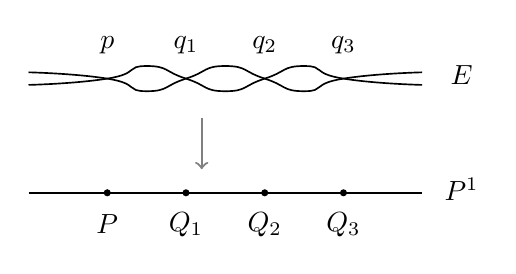
\begin{tikzpicture}[semithick]
  \draw plot[smooth,tension=1] coordinates {(0,0.08) (1,0) (1.5,-0.16) (2,0) (2.5,0.16) (3,0) (3.5,-0.16) (4,0) (5,0.08)};
  \draw plot[smooth,tension=1] coordinates {(0,-0.08) (1,0) (1.5,0.16) (2,0) (2.5,-0.16) (3,0) (3.5,0.16) (4,0) (5,-0.08)};
  \node at (1,0.42) {$p$};
  \node at (2,0.42) {$q_1$};
  \node at (3,0.42) {$q_2$};
  \node at (4,0.42) {$q_3$};
  \node at (5.5,0.05) {$E$};
  \draw[gray,thick,->] (2.2,-0.5) -- (2.2,-1.15);
  \draw (0,-1.45) -- (5,-1.45);
  \fill (1,-1.45) circle (0.045);
  \fill (2,-1.45) circle (0.045);
  \fill (3,-1.45) circle (0.045);
  \fill (4,-1.45) circle (0.045);
  \node at (1,-1.85) {$P$};
  \node at (2,-1.85) {$Q_1$};
  \node at (3,-1.85) {$Q_2$};
  \node at (4,-1.85) {$Q_3$};
  \node at (5.5,-1.4) {$\mathbb{P}^1$};
\end{tikzpicture}
\caption{\trEllipticCurve{}给出射影直线的二重覆盖，在四个点处分支（\S19.9.5）。（依原书手绘图重绘。）}\label{fig:genus1-double-cover}
\end{figure}

\textbf{19.9.6.}\ \emph{后续注记。}\quad 带有\textbf{完全水平 $n$ 结构}（full level $n$ structure）的\trEllipticCurve，是指一条\trEllipticCurve{}连同其 $n$-挠点与 $(\mathbb{Z}/n)^2$ 的一个\trIsomorphism。（若 $n$ 被 $\operatorname{char}k$ 整除，这个概念便会有问题。）于是，带完全水平 $2$ 结构的\trEllipticCurve，与其\trDegree{} $2$ 覆盖描述中给三个其余分支点取定一个排序的\trEllipticCurve，是同一回事。于是（若 $k=\bar{k}$）这些对象由 $\lambda$-直线参数化，我们将在下文讨论它。

\emph{后续的后续。}\quad 带完全水平 $n$ 结构的\trEllipticCurve{}的\trModuliSpace{}这一概念是存在的。这样的\trModuliSpace{}都是\trSmooth{}的\trCurve（在对这句话作恰当解读的意义上——它们是\trStack），并且具有\trSmooth{}的紧化。一个权为 $k$、水平为 $n$ 的\textbf{\trModularForm}（modular form）是 $\omega_M^{\otimes k}$ 的一个\trSection，其中 $\omega_M$ 是这个\trModuliSpace{}的\trCanonical{}层（这个\trModuliSpace{}称作「\textbf{\trModularCurve}」（modular curve））。

\textbf{19.9.7.}\ \emph{\trCrossRatio{}与 $j$-不变量。}\quad （我们保持 $k$ \trAlgClosed{}且特征不为 $2$ 的假设。）若把三个其余的分支点暂时标记为 $Q_1$、$Q_2$、$Q_3\in\mathbb{P}^1$，则有唯一的 $\mathbb{P}^1$ 的\trAutomorphism{}把 $P$、$Q_1$、$Q_2$ 依次送到 $\infty$、$0$、$1$（因为 $\Aut\mathbb{P}^1$ 是 $3$-可迁的，\mbox{练习~15.5.B}）。设在这个映射下 $Q_3$ 被送到某个数 $\lambda$，这里 $\lambda$ 必然不是 $0$、$1$、$\infty$。这个 $\lambda$ 值便称为 $\mathbb{P}^1$ 中四点 $(P,Q_1,Q_2,Q_3)$ 的\textbf{\trCrossRatio}（cross-ratio）（由\trn{Pappus of Alexandria}{亚历山大的帕普斯}所发明，[MO152008]）。

\textbf{19.9.B.（练习）}\quad 证明：$\mathbb{P}^1$ 上四个有序的互不相同的（闭）点（在\trAlgClosedField{} $k$ 上）的同构类，在模掉射影等价（$\mathbb{P}^1$ 的\trAutomorphism）的意义下，由\trCrossRatio{}分类。

\textbf{19.9.C.（练习）}\quad 证明：$(a,b,c,d)$ 的\trCrossRatio{}与 $(b,a,d,c)$ 的\trCrossRatio{}相同。群 $S_4$ 作用在 $\mathbb{P}^1$ 上点的四元组上，从而也作用在它们的\trCrossRatio{}上。证明：$S_4$ 在\trCrossRatio{}上的作用限制到「\trKlein{}四元群」$V_4\subset S_4$ 上时是平凡的。

我们尚未定义\emph{\trModuliSpace}的概念，但上一道练习例示了这样一个事实：$\mathbb{P}^1\setminus\{0,1,\infty\}$（\trCrossRatio{}映射的像）是 $\mathbb{P}^1$ 上四个有序的互不相同点模掉射影等价的\trModuliSpace。

注意：
\begin{itemize}[leftmargin=2.6em,itemsep=2pt,topsep=3pt]
\item 若我们改为把 $P$、$Q_2$、$Q_1$ 送到 $(\infty,0,1)$，则 $Q_3$ 就会被送到 $1-\lambda$。
\item 若我们改为把 $P$、$Q_1$、$Q_3$ 送到 $(\infty,0,1)$，则 $Q_2$ 就会被送到 $1/\lambda$。
\item 若我们改为把 $P$、$Q_3$、$Q_1$ 送到 $(\infty,0,1)$，则 $Q_2$ 就会被送到 $1-1/\lambda=(\lambda-1)/\lambda$。
\item 若我们改为把 $P$、$Q_2$、$Q_3$ 送到 $(\infty,0,1)$，则 $Q_1$ 就会被送到 $1/(1-\lambda)$。
\item 若我们改为把 $P$、$Q_3$、$Q_2$ 送到 $(\infty,0,1)$，则 $Q_1$ 就会被送到 $1-1/(1-\lambda)=\lambda/(\lambda-1)$。
\end{itemize}

于是，这六个值（它们对应于置换 $Q_1$、$Q_2$、$Q_3$ 的对称群 $S_3$）给出同一条\trEllipticCurve，而这条\trEllipticCurve（在对其余三个分支点取定一个排序之后）也将给出这六个值之一。

这已经相当令人满意了。要检验 $k=\bar{k}$ 上的两条\trEllipticCurve{} $(E,p)$ 与 $(E',p')$ 是否\trIsomorphic，我们把二者分别写成在 $p$ 与 $p'$ 处分歧的 $\mathbb{P}^1$ 的二重覆盖，然后给其余分支点排序，再分别计算各自的 $\lambda$（设为 $\lambda$ 与 $\lambda'$），看它们是否由上面六个表达式之一相互联系：
\begin{equation*}\tag{19.9.7.1}\label{eq:cross-ratio-six-values}
\lambda'=\lambda,\ 1/\lambda,\ 1-\lambda,\ 1/(1-\lambda),\ (\lambda-1)/\lambda,\ \text{或}\ \lambda/(\lambda-1).
\end{equation*}

如果代替这个「六值不变量」$\lambda$，存在单个的不变量（就叫它 $j$ 吧），使得 $j(\lambda)=j(\lambda')$ 当且仅当 \eqref{eq:cross-ratio-six-values} 中的等式之一成立，那将会远为方便。这个 $j$-函数想必应当是代数的，因此它会给出一个从 $\lambda$-直线 $\mathbb{A}^1\setminus\{0,1\}$ 到 $j$-直线 $\mathbb{A}^1$ 的映射 $j$。由\mbox{曲线到射影的延拓定理~15.3.1}，它将延拓成一个\trMorphism{} $j\colon\mathbb{P}^1\to\mathbb{P}^1$。由\mbox{练习~16.3.D}，由于这是（对大多数 $\lambda$ 而言）一个 $6$ 对 $1$ 的映射，这个覆盖的\trDegree{}为 $6$（或者更确切地说，至少为 $6$）。

我们可以把这个梦想按如下方式说得更精确。$k$ 上的椭圆曲线对应于 $\mathbb{P}^1\setminus\{0,1,\infty\}$ 的 $k$-值点，并模掉上面给出的 $S_3$ 在 $\lambda$ 上的作用。考虑 $k(\lambda)$ 中被 $S_3$ 固定的子域 $K$。那么扩张 $k(\lambda)/K$ 必然是 \trGalois{}的（例如见 [DF, \S14.2, Thm. 9]），且\trDegree{}为 $6$。我们希望这个子域形如 $k(j)$；若是这样，我们便会得到如上所述的 $j$-映射 $\mathbb{P}^1\to\mathbb{P}^1$。人们可以证明 $K$ 在 $k$ 上\trFinitelyGenerated，然后援引\trLuroth{}定理（我们很快将在\mbox{例~21.4.7}中证明它）；但我们并不需要这个。

不如我们就直接来搜寻这样的 $j$。注意 $\lambda$ 应当在 $k(j)$ 上满足一个六次多项式（或者，更精确地说，按我们此刻所知，满足一个\trDegree{}至少为 $6$ 的多项式），因为对每个 $j$-不变量，一般会有六个 $\lambda$ 值。

正如你毫无疑问已然知晓，这样的 $j$-不变量是存在的。下面就是人人都用的那个 $j$-不变量公式：
\begin{equation*}\tag{19.9.7.2}\label{eq:j-invariant-formula}
j=2^8\,\frac{(\lambda^2-\lambda+1)^3}{\lambda^2(\lambda-1)^2}.
\end{equation*}

你可以轻松验证 $j(\lambda)=j(1/\lambda)=j(1-\lambda)=\cdots$；并且由于 $j$（化成最简分式后）的分子\trDegree{}为 $6$、分母\trDegree{}小于 $6$，$j$ 的确决定了一个从 $\mathbb{P}^1$（以 $\lambda$ 为\trCoordinate）到 $\mathbb{P}^1$（以 $j$ 为\trCoordinate）的\trDegree{} $6$ 映射。但这个看起来很复杂的公式引出了一个问题：这个公式是从哪儿来的？当年的人是怎么想到它的？我们将在很大程度上回答这个问题，不过我们要把 $2^8$ 撇开不谈。正如你所想象的，这个 $2^8$ 来自特征 $2$ 的问题，而为了援引 \S19.5 的结果，我们一直假设 $\operatorname{char}k\ne 2$。（至于为什么在特征 $2$ 下这个 $2^8$ 是被迫加上的，见 [De, p. 64]。而从另一个复解析的视角看，$2^8$ 的由来是因为 $j$ 的 $q$-展开由 $j=q^{-1}+744+\cdots$ 开始：$q^{-1}$ 项的系数为 $1$；见 [Se5, p. 90, Rem. 2]。这两种看似不同的解释由\trTate{}曲线的理论联系在一起；见 [Si2, Thm. V.3.1]。）

与其使用这个白给的公式，不如让我们试着猜一猜 $j$ 是什么。我们不指望得到与 \eqref{eq:j-invariant-formula} 相同的公式，但我们的答案应当与它只相差 $j$-直线（$\mathbb{P}^1$）的一个\trAutomorphism——我们将得到 $j'=(aj+b)/(cj+d)$，其中 $a$、$b$、$c$、$d$ 为某组数（\mbox{练习~15.5.A}）。

我们要寻找某个 $j'(\lambda)$，使得 $j'(\lambda)=j'(1/\lambda)=\cdots$。于是我们想要某个在这个 $S_3$-作用之下不变的、含 $\lambda$ 的表达式。第一种可能的做法是取这六个数的乘积：
\[
\lambda\cdot(1-\lambda)\cdot\frac{1}{\lambda}\cdot\frac{\lambda-1}{\lambda}\cdot\frac{1}{1-\lambda}\cdot\frac{\lambda}{\lambda-1}.
\]
这就傻了，因为乘积显然等于 $1$。

一个好一些的想法是把它们统统加起来：
\[
\lambda+(1-\lambda)+\frac{1}{\lambda}+\frac{\lambda-1}{\lambda}+\frac{1}{1-\lambda}+\frac{\lambda}{\lambda-1}.
\]
这也不行，因为它们加起来是 $3$——这六项两两配对，每对的和都为 $1$。

（你或许会意识到这行不通的另一个理由：如果你审视这个和，你会意识到你将得到「\trDegree{}至多为 $3$」的东西除以「\trDegree{}至多为 $2$」的东西。那么，若 $j'=p(\lambda)/q(\lambda)$，则 $\lambda$ 在 $j$ 上是一个三次式的根。但我们说过 $\lambda$ 应当在 $j'$ 上满足一个六次式。避免矛盾的唯一办法是 $j'\in k$。）

但你毫无疑问马上就会有另一个主意。一个好主意是取这六个根的第二个对称函数。一个等价而更易于徒手演算的做法，是把这六项的平方加起来。甚至在动手计算之前，我们就能看出这招会灵：它显然会产出一个分子与分母\trDegree{}至多为 $6$ 的分式，并且它不是常数——当 $\lambda$ 是某个固定的小的数值（比如说 $1/2$）时，平方和是某个小的实数；而当 $\lambda$ 是一个大的实数时，平方和将不得不是某个大的实数（不同于 $\lambda=1/2$ 时的值）。

当你徒手把这些平方加起来（这并不难）之后，你将得到
\[
j'=\frac{2\lambda^6-6\lambda^5+9\lambda^4-8\lambda^3+9\lambda^2-6\lambda+2}{\lambda^2(\lambda-1)^2}.
\]

的确 $k(j)\cong k(j')$：你可以（再次徒手）验证
\[
2j/2^8=\frac{2\lambda^6-6\lambda^5+12\lambda^4-14\lambda^3+12\lambda^2-6\lambda+2}{\lambda^2(\lambda-1)^2}.
\]

于是 $2j/2^8-j'=3$。

\textbf{19.9.8. \trDegree{} $3$ 的\trLineBundle{}（$\mathrm{Pic}^3(E)$）。}

在 \S19.9.5 关于\trDegree{} $2$ \trLineBundle{}的讨论中，我们为了援引\trRiemann--\trHurwitz{}公式而假设了 $\operatorname{char}k\ne 2$ 与 $k=\bar{k}$。在本小节中，我们将不带任何假设出发，并随需要陆续追加假设。这样你就会看到：在更弱的假设下，哪些部分结果仍然成立。

考虑\trDegree{} $3$ 的\trInvertibleSheaf{} $\OO_E(3p)$。由\trRiemannRoch{}（\eqref{eq:h0-high-degree}），
\[
h^0(E,\OO_E(3p))=\deg(3p)-g+1=3.
\]
由于 $\deg\OO_E(3p)>2g$，这就给出一个\trClosedEmbedding（\mbox{注记~19.2.11}与\mbox{练习~19.2.E}）。于是我们有一个闭嵌入 $E\hookrightarrow\mathbb{P}^2_k$，其像为一条三次\trCurve。此外，$\mathbb{P}^2_k$ 中有一条以重数 $3$ 与 $E$ 相交于点 $p$ 的直线，它对应于 $\OO(3p)$ 的那个恰在 $p$ 处以重数 $3$ 消失的\trSection。（平面内以至少 $2$ 的重数与一条\trSmooth\trCurve{}相交的直线是一条\trTangentLine；见\mbox{定义~13.3.3}。平面内以至少 $3$ 的重数与一条\trSmooth\trCurve{}相交的直线称为一条\textbf{\trFlex{}线}（flex line），而该点便是这条\trCurve{}的一个\textbf{\trFlex{}点}（flex point）或简称\textbf{\trFlex}（flex）。）（见图~\ref{fig:weierstrass-cubic}。）

\begin{figure}[htbp]
\centering
\begin{tikzpicture}[semithick]
  \draw[dotted] (0,0) circle (1.7);
  \node at (-2.5,1.35) {$\mathbb{P}^2$};
  \node at (-2.32,0.88) {（未按比例！）};
  \draw[dotted] (0,-1.7) -- (0,1.7);
  \draw[dotted] (-1.7,0) -- (1.7,0);
  \node at (-0.62,-1.28) {$x=0$};
  \node at (0.98,0.24) {$y=0$};
  \node at (2.2,-1.05) {$z=0$};
  \draw (-1.05,0) ellipse (0.32 and 0.18);
  \draw plot[smooth,tension=1] coordinates {(-0.3,2.02) (0,1.72) (0.32,1.28) (0.16,0.62) (0.06,0.18) (0.18,-0.28) (0.42,-0.9) (0.5,-1.36)};
  \fill (0,1.72) circle (0.04);
  \node at (0.32,1.92) {$p$};
\end{tikzpicture}
\caption{寻找一条\trEllipticCurve{}的\trn{Weierstrass}{魏尔斯特拉斯}三次曲线化身。（依原书手绘图重绘。）}\label{fig:weierstrass-cubic}
\end{figure}

在 $\mathbb{P}^2_k$ 上选取射影\trCoordinate，使得 $p$ 被送到 $[0,1,0]$，而\trFlex{}线正是无穷远线 $z=0$。那么这条三次曲线便呈如下形状：
\[
\begin{aligned}
&?\,x^3\;\;+\;\;0\,x^2y\;\;+\;\;0\,xy^2\;\;+\;\;0\,y^3\\
&+\;\;?\,x^2z\;\;+\;\;?\,xyz\;\;+\;\;?\,y^2z\qquad\qquad\qquad=\ 0.\\
&\qquad+\;\;?\,xz^2\;\;+\;\;?\,yz^2\\
&\qquad\qquad+\;\;?\,z^3
\end{aligned}
\]

$x^3$ 的系数不是 $0$（否则这条三次曲线将被 $z$ 整除）。把整个方程除以这个系数，我们便可设 $x^3$ 的系数为 $1$。$y^2z$ 的系数也不是 $0$（否则这条三次曲线在 $x=z=0$ 处\trSingular）。我们可以缩放 $z$（即把 $z$ 换成它的一个适当的倍数），使得 $y^2z$ 的系数为 $-1$。若 $k$ 的特征不是 $2$，那么我们接着可以把 $y$ 换成 $y+?x+?z$，使得 $xyz$ 与 $yz^2$ 的系数为 $0$；而若 $k$ 的特征不是 $3$，我们便可以把 $x$ 换成 $x+?z$，使得 $x^2z$ 的系数也为 $0$。总之，若 $\operatorname{char}k$ 不是 $2$ 或 $3$，这条\trEllipticCurve{}便可以写成
\begin{equation*}\tag{19.9.8.1}\label{eq:weierstrass-normal-form}
y^2z=x^3+axz^2+bz^3.
\end{equation*}
这称为这条曲线的\textbf{\trWeierstrassNormalForm}（Weierstrass normal form）。

\textbf{19.9.9.}\ \emph{从\trn{Weierstrass}{魏尔斯特拉斯}三次曲线到二重覆盖。}\quad 令 $z=1$，或者更精确地说，在特异开集 $z\ne 0$ 中使用非齐次\trCoordinate{}工作，我们便看到这条曲线的超椭圆（二重覆盖）描述。下面就是三次曲线描述中何以能看见二重覆盖描述的几何解释。从 $p=[0,1,0]$ 出发投射这条三次曲线（见图~\ref{fig:weierstrass-to-double-cover}）。这是一个映射 $E\setminus p\to\mathbb{P}^1$（由 $[x,y,z]\mapsto[x,z]$ 给出），它基本上就是这条三次曲线到 $x$-轴的竖直\trProjection。（图~\ref{fig:weierstrass-to-double-cover}或许有助于你想见这个画面。）由\mbox{曲线到射影的延拓定理~15.3.1}，\trMorphism{} $E\setminus p\to\mathbb{P}^1$\footnote{原书此处作『$E-p$』，当为『$E\setminus p$』之误，径改。——译者注}可延拓到 $p$ 之上。若 $\mathscr{L}:=\OO(3p)$ 是给出这个\trMorphism{} $E\hookrightarrow\mathbb{P}^2$ 的\trLineBundle（经由\mbox{定理~15.2.2}——它以\trLineBundle{}的语言描述到射影空间的映射），那么给出到 $\mathbb{P}^1$ 的映射的那两个\trSection{} $x$ 与 $z$ 分别在 $p$ 处以 $1$ 阶与 $3$ 阶消失。为了把这个\trRationalMap{}「解消」成一个名副其实的\trMorphism，我们把 $x$ 与 $z$ 解释为 $\mathscr{L}(-p)=\OO(2p)$ 的\trSection，于是它们生成一个\trBasePointFree\trLinearSystem，从而生成一个到 $\mathbb{P}^1$ 的\trMorphism。（你或许能把这解读为用另一种语言实现\mbox{定理~15.2.2} 的证明。）类似的想法——施于四次曲线而非三次曲线——曾在\mbox{练习~19.7.C} 中得到使用。

\begin{figure}[htbp]
\centering
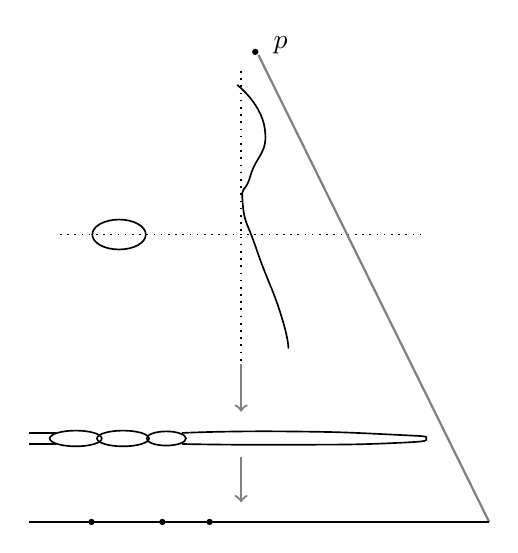
\begin{tikzpicture}[semithick]
  \draw[dotted] (0,-2.5) -- (0,1.2);
  \draw[dotted] (-2.3,-0.9) -- (2.3,-0.9);
  \draw (-1.55,-0.9) ellipse (0.34 and 0.19);
  \draw plot[smooth,tension=1] coordinates {(-0.05,1.0) (0.3,0.45) (0.12,-0.15) (0.02,-0.5) (0.2,-1.1) (0.5,-1.9) (0.6,-2.35)};
  \fill (0.18,1.42) circle (0.04);
  \node at (0.5,1.5) {$p$};
  \draw[gray,thick] (0.22,1.38) -- (3.15,-4.55);
  \draw[gray,thick,->] (0,-2.55) -- (0,-3.15);
  \draw (-2.7,-3.42) -- (-2.35,-3.42);
  \draw (-2.7,-3.56) -- (-2.35,-3.56);
  \draw (-2.1,-3.49) ellipse (0.33 and 0.10);
  \draw (-1.5,-3.49) ellipse (0.33 and 0.10);
  \draw (-0.95,-3.49) ellipse (0.25 and 0.09);
  \draw plot[smooth,tension=1] coordinates {(-0.75,-3.42) (0.5,-3.40) (1.9,-3.44) (2.35,-3.49) (1.9,-3.55) (0.5,-3.57) (-0.75,-3.56)};
  \draw[gray,thick,->] (0,-3.72) -- (0,-4.3);
  \draw (-2.7,-4.55) -- (3.15,-4.55);
  \fill (-1.9,-4.55) circle (0.04);
  \fill (-1.0,-4.55) circle (0.04);
  \fill (-0.4,-4.55) circle (0.04);
\end{tikzpicture}
\caption{从\trn{Weierstrass}{魏尔斯特拉斯}三次曲线到\trEllipticCurve{}的二重覆盖解读（参看图~\ref{fig:weierstrass-cubic}）。（依原书手绘图重绘。）}\label{fig:weierstrass-to-double-cover}
\end{figure}

作为一个推论，只要费上一点汗水，我们就能把 $j$-不变量计算为 $a$ 与 $b$ 的函数：
\[
j(a,b)=\frac{2^8\,3^3\,a^3}{4a^3+27b^2}.
\]

\textbf{19.9.D.（练习）}\quad 证明：这条三次曲线的诸\trFlex{}点恰好是群 $E$ 中的 $3$-挠点。（「\trFlex」的定义见 \S19.9.8：它是切线与曲线在该点以至少 $3$ 的重数相交的那个点。事实上，若 $k$ \trAlgClosed{}且 $\operatorname{char}k\ne 3$，它们共有九个。如果你熟悉复数的故事——$E\cong\mathbb{C}/\Lambda$——这不会令你惊讶。）

\textbf{19.9.10. 群律，几何地。}

这个群律有一个借助\trn{Weierstrass}{魏尔斯特拉斯}形式的优美的经典描述。参看图~\ref{fig:group-law-geometric}。在\trn{Weierstrass}{魏尔斯特拉斯}\trCoordinate{}下，原点 $p$ 是 $E$ 与无穷远线（$z=0$）相交的唯一一点；事实上，无穷远线对应于 $\OO(3p)$ 的重言截面。若一条直线与 $E$ 相交于三点 $p_1$、$p_2$、$p_3$，则
\[
\OO(p_1+p_2+p_3)\cong\OO(3p),
\]
从而（在群律中）$p_1+p_2+p_3=0$。

于是，为求一个点 $s$ 的逆，我们考虑 $E$ 与直线 $\overline{sp}$ 的交：$-s$ 就是第三个交点。为求两点 $q$ 与 $r$ 的和，我们考虑 $E$ 与直线 $\overline{qr}$ 的交，并把第三个交点称为 $s$。然后我们通过把 $s$ 与 $p$ 相连来计算 $-s$，从而得到 $q+r$。

\begin{figure}[htbp]
\centering
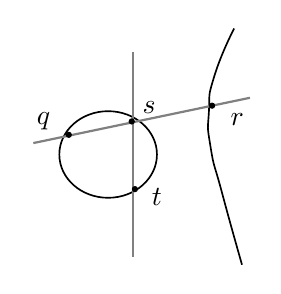
\begin{tikzpicture}[semithick]
  \draw (0,0) ellipse (0.62 and 0.55);
  \draw plot[smooth,tension=1] coordinates {(1.6,1.6) (1.35,1.0) (1.28,0.55) (1.3,0.1) (1.45,-0.5) (1.7,-1.4)};
  \draw[gray,thick] (0.32,-1.3) -- (0.32,1.3);
  \draw[gray,thick] (-0.95,0.145) -- (1.8,0.72);
  \fill (-0.5,0.25) circle (0.04);  \node at (-0.82,0.42) {$q$};
  \fill (0.30,0.42) circle (0.04);  \node at (0.52,0.60) {$s$};
  \fill (1.32,0.62) circle (0.04);  \node at (1.64,0.44) {$r$};
  \fill (0.34,-0.44) circle (0.04); \node at (0.62,-0.54) {$t$};
\end{tikzpicture}
\caption{\trEllipticCurve{}上的群律，几何地。（依原书手绘图重绘。）}\label{fig:group-law-geometric}
\end{figure}

我们可以把关于\trWeierstrassNormalForm{}中三次曲线之群律的这一番描述讲给任何熟悉射影空间概念与群概念的人听，但那样一来，我们就必须证明我们所给出的构造确实定义了一个群。特别地，我们将不得不证明结合律，而这并不是先验清楚的。但在眼下这个情形，我们已经通过给出到 $\mathrm{Pic}^0E$ 的一个\trBijection{}确立了\trDegree{} $1$ 点构成一个群，我们不过是在解读 $\mathrm{Pic}^0E$ 上的群律罢了。

注意，这一描述甚至在特征 $2$ 与特征 $3$ 时也有效；我们不需要这条三次曲线处于\trWeierstrassNormalForm，只需要 $\OO(3p)$ 给出一个到 $\mathbb{P}^2$ 的\trClosedEmbedding{}即可。

\textbf{19.9.11. \trDegree{} $4$ 的\trLineBundle。}\quad 你大概已经把这件事忘了：我们最初是按\trDegree{}一个一个地研究\trLineBundle{}的。这段故事到\trDegree{} $3$ 并不会止步。正如我们曾证明了\trGenus{} $4$ 的典范嵌入的非超椭圆\trCurve{}是 $\mathbb{P}^3_k$ 中一个二次曲面与一个三次曲面的\trCompleteIntersection（\S19.8），我们可以证明下面的结论。

\textbf{19.9.E.（练习）}\quad 证明：$\OO(4p)$ 的完全\trLinearSystem{}把 $E$ 嵌入 $\mathbb{P}^3$，使其像为两个二次曲面的\trCompleteIntersection。提示：证明 $E$ 的像包含在至少两个线性无关的二次曲面之中。证明二者都不可能是可约的（reducible），从而它们没有公共的\trIrreducibleComponent。仿照 \S19.8.1，使用\trBezout{}定理（\mbox{练习~18.6.J}）与\mbox{练习~18.6.E}。

这段优美的结构到\trDegree{} $4$ 还不会止步，但它变得更加复杂。例如，\trDegree{} $5$ 的嵌入不是一个\trCompleteIntersection（不是若干超曲面的交），而是 $G(2,5)$ 在其\trPluckerEmbedding{}之下与五个超平面的\trCompleteIntersection（或者，也许更好的说法是，与一个余维数为 $5$ 的\trLinearSpace{}的\trCompleteIntersection）。用看起来不同的术语来说，它的方程是一个一般的 $5\times 5$ 线性形式反对称矩阵（skew-symmetric matrix）的诸 $4\times 4$ 普法夫式（Pfaffians），不过我不会去说这是什么意思。（这个构造或许会让你想起 \S19.8.3 中对\trGenus{} $6$ \trCurve{}的一个类似构造。这绝非巧合。）


\section{\trEllipticCurve{}是\trGroupVariety}

\epigraph{自 1949 年以来，我一直把构造\trPicard{}簇的代数理论视为抽象代数几何中最为紧迫的任务。}{——A.~\trWeil，[Weil, p.~537]}

我们最初以一种相当抽象的方式描述了一条\trAlgebraic\trCurve{}上\trDegree{} $1$ 的点上的\trGroupLaw。从那个定义出发，看不出在 $\mathbb{C}$ 上群运算（加法、求逆）是连续的。而用\trn{Weierstrass}{魏尔斯特拉斯}三次曲线作出的显式描述则把这一点弄清楚了。事实上，我们还能观察到更多：加法与求逆在一般情形下都是代数的。更好的是，\trEllipticCurve{}是\trGroupVariety。（因此它们是\trAbelianVariety；见\mbox{定义~11.4.11}。）

\textbf{19.10.1.}（这是一个线索：$\mathrm{Pic}^0(E)$ 打心底里想成为一个\trScheme，而不只是一个\trGroup。一旦「\trVariety{}上\trLineBundle{}的\trModuliSpace」这一概念被严格表述，这一点便可以得到证明；例如见 [FGIKNV, Part 5]。）

我们先从「群求逆」\trMorphism{}入手，作为热身。

\textbf{19.10.2.\ \trhProposition。}\ ——\ \emph{若 $\operatorname{char}k\ne 2$、$3$，则存在一个 $k$-簇的\trMorphism{} $E\to E$，把（\trDegree{} $1$ 的）点送到它的逆元，并且这一构造在 $k$ 的\trFieldExtension{}之下表现良好。}

但换言之，\trGroupLaw{}中的「求逆映射」其实来自一个概形的\trMorphism——它不只是一个集合映射。（欢迎你自行把剩下的两种\trCharacteristic{}想一想，并看到本质相同的证明照样适用。\mbox{定理~19.10.4} 的证明会让你更好地知道该如何着手。）

\emph{证明。}\quad 考虑\trn{Weierstrass}{魏尔斯特拉斯}范式的映射（超椭圆对合）$y\mapsto -y$。\hfill$\square$

加法的代数描述若要显式写下来，将会是一团乱麻。我们将能凭一个技巧来证明代数性——不是把它显式地写出来，而是想清楚我们如何\emph{能够}把它显式地写出来。这个技巧的主要部分是下面的\trhProposition。我们把它表述得稍许一般，只因它可能有用；但你或许更愿意假设 $k=\bar{k}$ 且 $C$ 是一条\trRegular{}的三次曲线。若 $C$ 是一条\trCurve，令 $C^{\mathrm{reg}}$ 为 $C$ 的\trRegular{}点，或者等价地，\trNormal{}点（\mbox{定理~13.5.8}），它们构成 $C$ 的一个\trOpenSubset（\mbox{练习~10.7.O}）。

\textbf{19.10.3.\ \trhProposition。}\ ——\ \emph{设 $C\subset\mathbb{P}^2_k$ 是一条\trGeometricallyIntegral{}的三次\trCurve（故特别地，$C$ 不含直线）。存在唯一的\trMorphism{} $t\colon C^{\mathrm{reg}}\times C^{\mathrm{reg}}\to C^{\mathrm{reg}}$，使得}
\begin{itemize}
\item[\emph{(a)}] \emph{若 $p$ 与 $q$ 是 $C$ 上两个互不相同的正则 $k$-\trValuedPoint，则 $t(p,q)$ 如此得到：以直线 $\overline{pq}$ 与 $C$ 相交，取其与 $C$ 相交的第三个「剩余」点。更精确地说，$\overline{pq}$ 将计重数与 $C$ 交于三点（\mbox{练习~9.3.D}），其中含 $p$ 与 $q$；$t(p,q)$ 即第三个点；且}
\item[\emph{(b)}] \emph{这一性质在扩张到 $\bar{k}$ 之后仍然成立。}
\end{itemize}
\emph{此外，若 $p$ 是 $C^{\mathrm{reg}}$ 的一个 $k$-\trValuedPoint，则 $t(p,p)$ 就是 $C$ 在 $p$ 处的\trTangentLine{} $\ell$ 再次与 $C$ 相交之处。更精确地说，$\ell$ 将计重数与 $C$ 交于三点，其中 $p$ 以重数 $2$ 计入；$t(p,p)$ 即第三个点。}

我们需要性质 (b)，因为 $C$ 的 $k$-\trValuedPoint{}可能少得可怜（甚至一个也没有！），以至于\trMorphism{} $t$ 无法由它在这些点上的行为所确定。在证明的进程中，我们将看到 (b) 可以扩充为「这一性质在 $k$ 的任何\trFieldExtension{}之后仍然成立」。

\emph{证明。}\quad 我们先（在本段中）证明：若 $p$ 与 $q$ 是两个互不相同的\trRegular{}点，则 $\overline{pq}$ 与 $C$ 的第三个交点 $r$ 也是\trRegular{}的。若 $r=p$ 或 $r=q$，则已然证毕。否则，把 $C$ 限制到 $\overline{pq}$ 上所得的三次式有三个互不相同的根 $p$、$q$、$r$（从而既约，即重数为 $1$）。于是 $C\cap\overline{pq}$ 在 $r$ 处是\trRegular{}的，故由正则性的\trSlicing{}判别法（\mbox{练习~13.2.C}），$r$ 是 $C$ 的一个\trRegular{}点。

现在我们假设 $k=\bar{k}$，并把一般情形留到最后。固定 $p$、$q$、$r$，其中 $p\ne q$，而 $r$ 是 $\overline{pq}$ 与 $C$ 的「第三」个交点。我们将描述 $(p,q)\in C^{\mathrm{reg}}\times C^{\mathrm{reg}}$ 的一个开邻域内的\trMorphism{} $t_{p,q}$。由\mbox{练习~11.3.B}——它断言 $\bar{k}$ 上\trVariety{}的\trMorphism{}由其在闭（$\bar{k}$-值）点上的行为所确定——这些\trMorphism（唯一地）相互粘合，给出一个\trMorphism{} $t$，至此 $k=\bar{k}$ 情形的证明便完成了。

在 $\mathbb{P}^2$ 上选取\trProjective\trCoordinate，使得 $U_0\cong\Spec k[x_1,x_2]$ 包含 $p$、$q$、$r$，且直线 $\overline{pq}$ 不「竖直」。更精确地说，在 $\Spec k[x_1,x_2]$ 中，说 $p=(p_1,p_2)$（用「经典坐标」的话说——更学究气一点，$p=[(x_1-p_1,\ x_2-p_2)]$），$q=(q_1,q_2)$，$r=(r_1,r_2)$，且 $p_1\ne q_1$。在这些\trCoordinate{}下，\trCurve{} $C$ 由某个三次式切出，我们也把它马虎地记作 $C$：$C(x_1,x_2)=0$。

现在设 $P=(P_1,P_2)$ 与 $Q=(Q_1,Q_2)$ 是 $C\cap U_0$ 的两个点（不必是我们的 $p$ 与 $q$）。我们尝试计算 $\overline{PQ}$ 与 $C$ 的第三个交点，且要算得能在 $C\times C$ 的一个包含 $(p,q)$ 的开子集上通行。显式地做这件事需要丑陋的高中代数；但正因为我们知道它长什么样子，我们才能够避开一切细节！

直线 $\overline{PQ}$ 由 $x_2=mx_1+b$ 给出，其中 $m=\frac{P_2-Q_2}{P_1-Q_1}$ 与 $b=P_2-mP_1$ 都是 $P$ 与 $Q$ 的\trRationalFunction。于是，对一切满足 $P_1\ne Q_1$ 的 $P$ 与 $Q$，$m$ 与 $b$ 都有定义（从而在 $(p,q)$ 的一个开邻域上有定义，因为 $p_1\ne q_1$，且 $P_1\ne Q_1$ 是一个开条件）。

现在我们求解 $C\cap\overline{PQ}$：把 $x_2=mx_1+b$ 代入 $C$，得到 $C(x_1,mx_1+b)$。这是 $x_1$ 的一个三次式，设为
\[
\gamma(x_1)=Ax_1^3+Bx_1^2+Cx_1+D=0.
\]
$\gamma$ 的系数是 $P_1$、$P_2$、$Q_1$、$Q_2$ 的\trRationalFunction。只要 $A\ne 0$，三次式 $\gamma$ 就有三个根（计重数），而这是一个关于 $m$ 与 $b$ 的\trZariski{}开条件，从而是关于 $P_1$、$P_2$、$Q_1$、$Q_2$ 的\trZariski{}开条件。由于 $P$、$Q\in C\cap\overline{PQ}\cap U_0$，$P_1$ 与 $Q_1$ 是 $\gamma(x_1)=0$ 的根中的两个。由于直线 $\overline{PQ}$ 包含 $p$、$q$、$r$，$\gamma(x_1)=0$ 的第三个根是 $R_1$\footnote{原书此处小写作「contains p, q, and r」而径接大写的「R$_1$」，两相抵牾；疑当为「$P$、$Q$ 与 $R$」（$R$ 即 $\overline{PQ}$ 与 $C$ 的第三个交点），兹照录原书。——译者注}。$\gamma(x_1)=0$ 诸根之和为 $-B/A$（由\trViete{}（Vi\`ete）公式），故 $\gamma$ 的第三个根是 $R_1:=-B/A-P_1-Q_1$。于是若取 $R_2=mR_1+b$，我们便找到了 $\overline{PQ}$ 与 $C$ 的第三个交点（可喜的是，它恰好落在 $U_0$ 中）。我们由此描述了一个从 $(C^{\mathrm{reg}}\cap U_0)\times(C^{\mathrm{reg}}\cap U_0)$ 的某个包含 $(p,q)$ 的开子集出发的\trMorphism，它所做的正是我们想要的。（精确地说，这个开子集由 $A\ne 0$ 定义，这一点可以被显式地解开。）至此，我们在 $k=\bar{k}$ 的情形完成了\mbox{命题~19.10.3} 的证明（除最后一段外）。（那些自认为只关心\trAlgClosedField{}的读者可以往下跳读。）

我们把上述构造扩充到除 $\mathbb{F}_2$ 之外的每一个域上的\mbox{命题~19.10.3}。设 $U_0^{[x_1,x_2]}=\Spec k[x_1,x_2]$ 是 $\mathbb{P}^2_k$ 的任意一个\trAffine\trOpenSubset，连同\trCoordinate{}的选取。（这个别扭的上标 $[x_1,x_2]$ 是为了强调：构造中使用的是这一组特定的\trCoordinate。）于是，上面的构造给出一个\emph{定义于 $k$ 上}的\trMorphism，其定义域是 $(C^{\mathrm{reg}}\cap U_0^{[x_1,x_2]})\times(C^{\mathrm{reg}}\cap U_0^{[x_1,x_2]})$ 的一个开子集（注意，所有这套假想中进行的代数演算都是在 $k$ 上做的），它把 $P$ 与 $Q$ 送到 $\overline{PQ}$ 与 $C$ 的第三个交点。注意这一构造与任何\trFieldExtension{}交换，因为这个构造对我们所工作的域并不敏感。于是，换基到\trAlgebraicClosure{}之后，这个映射也具有如下性质：以两个点为输入，吐出直线与三次曲线的第三个交点。此外，所有这些映射（当 $U_0^{[x_1,x_2]}$ 取遍「以 $k$ 为系数的」直线的补集 $U_0$ 连同 $U_0$ 上\trCoordinate{}的各种选取时）可以粘合在一起：它们在两两重叠处一致（因为换基到 $\bar{k}$ 之后它们是同一个映射，这由前面的讨论可知；而换基到 $\bar{k}$ 之后相同的两个映射本来就是相同的，见\mbox{练习~10.2.J}），而这正是把它们粘合起来所需要的（\mbox{练习~7.2.A}）。

我们可以通过检视这一构造，来几何地解读开子集 $(C^{\mathrm{reg}}\cap U_0^{[x_1,x_2]})\times(C^{\mathrm{reg}}\cap U_0^{[x_1,x_2]})$：它定义在轨迹 $\{P=(P_1,P_2),\ Q=(Q_1,Q_2)\}$ 之上，其中 (i) $P_1\ne Q_1$，且 (ii) $\overline{PQ}$ 与 $C$ 的第三个交点 $R$ 也落在 $U_0$ 中。

那么，$C^{\mathrm{reg}}\times C^{\mathrm{reg}}$ 中哪些点 $(P,Q)$ 被漏掉了？最重要的：我们漏掉了 $P=Q$ 的情形。

\textbf{19.10.A.（练习）}\quad 用\mbox{扩展例题~15.3.4} 的代数来处理 $P=Q$ 的情形。（这会花去一些时间与细心。理想情况下，你应当避免做任何脏乱的代数。）

我们现在来处理剩下的 $P\ne Q$ 的情形。条件 (i) 并不重要：若 $(P,Q)$ 满足 (ii) 而不满足 (i)，我们可以对换 $x_1$ 与 $x_2$ 的角色，$(P,Q)$ 便转而满足 (i)。$(P,Q)$ 不能被这些开集之一覆盖的唯一方式，是\emph{不存在}把 $P$、$Q$、$R$ 三点都包含进去的 $U_0$（某条定义于 $k$ 上的直线的补集）。

\textbf{19.10.B.（练习）}\quad 利用 $|k|>2$ 证明：$\mathbb{P}^2$ 上存在一个系数取于 $k$ 的线性形式，它避开 $P$、$Q$、$R$ 三点。（遗憾的是，当 $k=\mathbb{F}_2$ 时这\emph{不}真——你明白为什么吗？）

\textbf{19.10.C.（练习）}\quad 证明\mbox{命题~19.10.3} 的最后一个论断。

\textbf{19.10.D.}\ \extrahard\ \textbf{（不重要练习）}\quad 通过处理 $k=\mathbb{F}_2$ 的情形来完成证明。提示：先在 $\mathbb{F}_4$ 上造出\trMorphism{} $t$。目标随即是证明这个 $t$ 其实「定义于」$\mathbb{F}_2$ 之上（「下降到」$\mathbb{F}_2$）。这个\trMorphism{} $t$ 最初是这样局部地描述的：考虑一条定义于 $\mathbb{F}_4$ 上的直线的补集（然后让这条直线变动）。不妨换一种方式：转而考察一条直线及其「共轭」直线的补集，从中盯着这个映射看。这条直线与其共轭的补集是一个仿射 $\mathbb{F}_2$-\trVariety。这个仿射\trVariety{}上部分定义的映射 $t$ 先验地定义于 $\mathbb{F}_4$ 之上，并且在共轭之下保持。证明这个部分定义的映射「真正」定义于 $\mathbb{F}_2$ 之上。（如果你把这一切的含义都想明白了，你就已经对「\trDescent」理论有了重要的初识。）

\begin{flushright}$\square$\end{flushright}

现在我们可以用这个来定义 $E$ 上的\trGroupVariety{}结构了。

\textbf{19.10.4.\ \trhTheorem。}\ ——\ \emph{设 $(E,p)$ 是一条\trEllipticCurve（$k$ 上一条\trRegular{}的\trGenus{} $1$ \trCurve，带有一个 $k$-\trValuedPoint{} $p$）。取 $E$ 在 $\mathbb{P}^2_k$ 中经由完全\trLinearSystem{} $|\OO_E(3p)|$ 的\trn{Weierstrass}{魏尔斯特拉斯}嵌入。定义 $k$-\trMorphism{} $e\colon\Spec k\to E$ 为把 $\Spec k$ 送到 $p$。定义 $k$-\trMorphism{} $i\colon E\to E$ 为 $q\mapsto t(p,q)$，或者更精确地说，作为复合}
\[
\begin{tikzcd}
E \ar[r, "{(\id,e)}"] & E\times E \ar[r, "t"] & E.
\end{tikzcd}
\]
\emph{定义 $k$-\trMorphism{} $m\colon E\times E\to E$ 为 $(q,r)\mapsto t(p,t(q,r))$。则 $(E,e,i,m)$ 是 $k$ 上的一个\trGroupVariety。}

由 $t$ 的构造，这些\trMorphism{}全都「与任意基扩张交换」。

\emph{证明。}\quad 我们需要验证 \S7.6.4 的公理 (i)--(iii) 中所述的各种态射对相等。例如，在公理 (iii) 中，我们需要证明 $m\circ(i,\id)=m\circ(\id,i)$；所有公理显然都属于这种类型。

先设 $k=\bar{k}$。这时，每一对态射作为 $\bar{k}$-点的映射都是一致的：$\mathrm{Pic}\,E$ 是一个群，而沿着\mbox{命题~19.9.3} 给出的 $\mathrm{Pic}\,E$ 与 $E$ 之间的\trBijection，再借助 \S19.9.10 的讨论，群运算恰好翻译成\mbox{定理~19.10.4} 论断中所描述的那些映射。

但 $\bar{k}$-\trVariety{}的\trMorphism{}由其在 $\bar{k}$-点层面上的映射所决定（\mbox{练习~11.3.B}），故每一对态射都是相同的。

对一般的 $k$，我们注意到，由 $\bar{k}$ 的情形可知，这些态射在换基到\trAlgebraicClosure{}之后是一致的。于是由\mbox{练习~10.2.J}，它们本来就是一致的。\hfill$\square$

\textbf{19.10.5.}\ \emph{这一构造的诸特色。}\quad 关于\trEllipticCurve{}的性质，最常见的推导方式是把椭圆曲线描述为一条三次曲线，再用与直线的显式构造来描述加法。然后人们还得费力去证明所描述的乘法是结合的。

我们的做法则相反：从一个明摆着就是群的东西（\trDegree{}为 $0$ 的\trLineBundle）出发。我们利用椭圆曲线的三次曲线解读，几何地解读了群的定义中所用的那些映射（加法与求逆）。这使我们得以看出这些映射是代数的。

作为附带收获，我们看到：在某种模糊的意义上，椭圆曲线的\trPicardGroup{}想要成为一个\trAlgebraic\trVariety。

\textbf{19.10.E.（练习）}\quad 设 $p$ 与 $q$ 是一条\trGenus{} $1$ \trCurve{} $E$ 的两个 $k$-点。证明 $E$ 有一个把 $p$ 送到 $q$ 的\trAutomorphism。

\textbf{19.10.F.（练习）}\quad 设 $(E,p)$ 是\trCharacteristic{}不为 $2$ 或 $3$ 的\trAlgClosedField{} $k$ 上的一条\trEllipticCurve。证明 $(E,p)$ 的\trAutomorphismGroup\trIsomorphic{}于 $\mathbb{Z}/2$、$\mathbb{Z}/4$ 或 $\mathbb{Z}/6$。（$k=\bar{k}$ 时，椭圆曲线 $(E,p)$ 的一个\trAutomorphism{}是指概形论地固定 $p$ 的 $E$ 的\trAutomorphism，或者等价地，由\mbox{练习~11.3.B}，固定 $k$-\trValuedPoint{} $p$。）提示：化归到 $\mathbb{P}^1$ 的、固定一个点 $\infty$ 与三个互不相同之点的集合 $\{p_1,p_2,p_3\}\in\mathbb{P}^1\setminus\{\infty\}$ 的\trAutomorphism{}这一问题\footnote{原书此处集合记号作「$\{p_1,p_2,p_3\}\in\mathbb{P}^1\setminus\{\infty\}$」，疑当为「$\subset$」，兹照录原书。——译者注}。（$k$ 的代数闭并不关键，尽可利用\mbox{练习~10.2.J} 去掉这一假设。如果\trCharacteristic{}是 $3$ 会怎样？）

\textbf{19.10.G.（练习）}\quad 解释为什么\trCharacteristic{}不为 $2$ 的\trAlgClosedField{}上的\trGenus{} $1$ \trCurve{}由 $j$-不变量分类（在\trIsomorphism{}的意义下）。（当心：注意题目说的是「\trGenus{} $1$」，而不是「椭圆」。）

\textbf{19.10.H.（练习）}\quad 给出（连同证明）$\mathbb{Q}$ 上两条具有相同 $j$-不变量却互不\trIsomorphic{}的\trEllipticCurve。（提示：\S19.5.3。）

\textbf{19.10.6.}\ \emph{模糊问题。}\quad \trCharacteristic{}不为 $2$ 的\trAlgClosedField{} $k$ 上的\trGenus{} $1$ \trCurve，其可能的\trAutomorphismGroup{}有哪些？你应当能让自己相信这个群具有「维数 $1$」。

\textbf{19.10.I.（重要练习：一条退化的\trEllipticCurve）}\quad 设 $\operatorname{char}k\ne 2$。考虑算术\trGenus{}为 $1$ 的\trCurve{} $C\subset\mathbb{P}^2_k$，由 $y^2z=x^3+x^2z$ 给出，并带有点 $p=[0,1,0]$。模仿上面的论证，证明 $C\setminus\{[0,0,1]\}$ 是一个\trGroupVariety（其中的运算是由\trLineBundle{}的张量给出的那个运算）。证明它\trIsomorphic{}于 $\mathbb{G}_m$（\trMultiplicativeGroup{}概形 $\Spec k[t,t^{-1}]$；见\mbox{练习~7.6.E}），坐标为 $t=(y-x)/(y+x)$；做法是给出一个概形的\trIsomorphism，并证明两个\trGroupVariety{}中的乘法与求逆在这个\trIsomorphism{}之下相吻合。

\textbf{19.10.J.（练习：一条更加退化的\trEllipticCurve）}\quad 考虑算术\trGenus{}为 $1$ 的\trCurve{} $C\subset\mathbb{P}^2_k$，由 $y^2z=x^3$ 给出，并带有点 $p=[0,1,0]$。模仿上面的论证，证明 $C\setminus\{[0,0,1]\}$ 是一个\trGroupVariety（其中的运算是由\trLineBundle{}的张量给出的那个运算）。证明它\trIsomorphic{}于 $\mathbb{A}^1$（带有加法群结构），坐标为 $t=x/y$；做法是给出一个概形的\trIsomorphism，并证明两个\trGroupVariety{}中的乘法／加法与求逆在这个\trIsomorphism{}之下相吻合。

\textbf{19.10.7.}\ \hard\ \textbf{通向\trPoncelet{}衍论。}

这些想法引出一个漂亮的经典事实——\trPoncelet{}（Poncelet）衍论（porism）。（「衍论」是对某一类数学结果的古称。）

\begin{figure}[htbp]
\centering
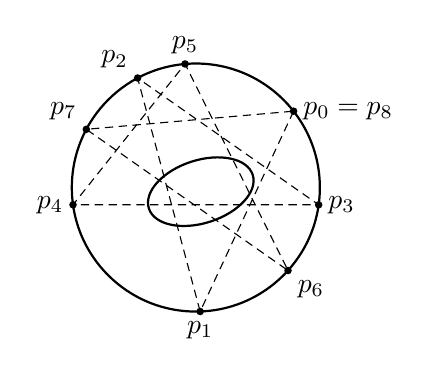
\begin{tikzpicture}[scale=1.05]
\draw[thick] (0,0) circle (1.5);
\begin{scope}[shift={(0.06,-0.05)},rotate=18]
\draw[thick] (0,0) ellipse (0.66 and 0.38);
\end{scope}
\coordinate (p0) at (38:1.5);
\coordinate (p1) at (-88:1.5);
\coordinate (p2) at (118:1.5);
\coordinate (p3) at (-8:1.5);
\coordinate (p4) at (188:1.5);
\coordinate (p5) at (95:1.5);
\coordinate (p6) at (-42:1.5);
\coordinate (p7) at (152:1.5);
\draw[densely dashed] (p0) -- (p1) -- (p2) -- (p3) -- (p4) -- (p5) -- (p6) -- (p7) -- cycle;
\foreach \pt in {p0,p1,p2,p3,p4,p5,p6,p7} \fill (\pt) circle (1.3pt);
\node[above] at (p5) {$p_5$};
\node[right] at (p0) {$p_0=p_8$};
\node[right] at (p3) {$p_3$};
\node[below right] at (p6) {$p_6$};
\node[below] at (p1) {$p_1$};
\node[left] at (p4) {$p_4$};
\node[above left] at (p7) {$p_7$};
\node[above left] at (p2) {$p_2$};
\end{tikzpicture}
\caption{\trPoncelet{}衍论（\mbox{19.10.8}）。（依原书手绘图重绘。）}\label{fig:poncelet-porism}
\end{figure}

\textbf{19.10.8.\ \trPoncelet{}衍论。}\ ——\ \emph{设 $C$ 与 $D$ 是 $\mathbb{R}^2$ 中的两个椭圆，$C$ 包含 $D$。在 $C$ 上任取一点 $p_0$。从 $p_0$ 向 $D$ 引的两条切线中任取一条，记作 $\ell_1$。于是 $\ell_1$ 总共与 $C$ 交于两点：$p_0$ 与另外一个点 $p_1$。从 $p_1$ 出发，向 $D$ 有两条切线，$\ell_1$ 与另一条直线 $\ell_2$。直线 $\ell_2$ 与 $C$ 交于另一个点 $p_2$。如此继续下去，便得到一个点列 $p_0$、$p_1$、$p_2$、$\dots$。设这个以 $p_0$ 为起点的序列是周期的，即对某个 $n$ 有 $p_0=p_n$。那么，以任意一点 $p\in C$ 为起点，它都是周期的（见图~\ref{fig:poncelet-porism}）。}

\trPoncelet{}衍论存在初等的证法，但一个牵涉椭圆曲线的证明相当漂亮，并且与一些更精致的思想建立起联系。我们不去证明\trPoncelet{}衍论，而是讨论几个相关的事实。

\textbf{19.10.K.（练习）}\quad 设 $E$ 是\trAlgClosedField{}上一条\trSmooth{}的\trDegree{} $3$ 射影平面\trCurve，$q$、$r\in E$，而 $n$ 是一个正整数。令 $F\colon E\to E$ 是\trMorphism{} $x\mapsto t(r,t(q,x))$。设对某个\trClosedPoint{} $p\in E$ 有 $F^n(p)=p$。证明：对一切点 $x\in E$ 都有 $F^n(x)=x$。

你应当感到一股想要改进这个结果的冲动。（你能证明：若对某个 $p\in E$ 有 $F^n(p)=p$，则 $F^n$ 是 $E$ 上的\trIdMorphism{}吗？你能把它推广到\trBaseField{}不\trAlgClosed{}的情形吗？）

\textbf{19.10.L.（练习）}\quad 设 $E$ 是 $\mathbb{R}^2$ 中的一个椭圆。对每个点 $(x,y)\in E$，存在另外一个点 $G(x,y):=(x,y')$（可能与原来那个点相同），它具有相同的第一个坐标，对应于过 $(x,y)$ 的竖直线与 $E$ 的「另一个」交点。类似地，存在另外一个点 $H(x,y):=(x',y)$，它具有相同的第二个坐标。令 $F=G\circ H$。证明：若对某个点 $p\in E$ 有 $F^{17}(p)=p$，则对一切点 $x\in E$ 都有 $F^{17}(x)=x$。（见图~\ref{fig:ellipse-staircase}，其中把 $17$ 换成了 $3$。）提示：这最好不用任何来自代数几何的花哨方法来做。

再说一次，你应当盼望改进这一点。这在多大的程度上依赖于实数？如果椭圆换成了另外一种圆锥截线呢？（这与\trEllipticCurve{}又有什么关系？这条圆锥截线为什么叫 $E$？！）

\begin{figure}[htbp]
\centering
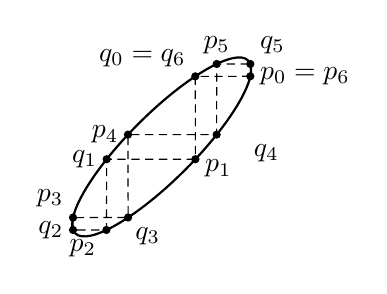
\begin{tikzpicture}[scale=1.15]
\begin{scope}[rotate=45]
\draw[thick] (0,0) ellipse (1.35 and 0.362);
\end{scope}
\coordinate (pa) at (0.979,0.780);
\coordinate (qa) at (0.371,0.779);
\coordinate (pb) at (0.372,-0.136);
\coordinate (qb) at (-0.607,-0.136);
\coordinate (pc) at (-0.610,-0.917);
\coordinate (qc) at (-0.979,-0.917);
\coordinate (pd) at (-0.979,-0.780);
\coordinate (qd) at (-0.371,-0.779);
\coordinate (pe) at (-0.372,0.136);
\coordinate (qe) at (0.607,0.136);
\coordinate (pf) at (0.608,0.916);
\coordinate (qg) at (0.979,0.916);
\draw[densely dashed] (pa) -- (qa) -- (pb) -- (qb) -- (pc) -- (qc) -- (pd) -- (qd) -- (pe) -- (qe) -- (pf) -- (qg) -- cycle;
\foreach \pt in {pa,qa,pb,qb,pc,qc,pd,qd,pe,qe,pf,qg} \fill (\pt) circle (1.3pt);
\node[right] at (pa) {$p_0=p_6$};
\node[above left] at (qa) {$q_0=q_6$};
\node[right, yshift=-0.12cm] at (pb) {$p_1$};
\node[left] at (qb) {$q_1$};
\node[below, xshift=-0.3cm] at (pc) {$p_2$};
\node[left] at (qc) {$q_2$};
\node[left, yshift=0.25cm] at (pd) {$p_3$};
\node[below, xshift=0.25cm] at (qd) {$q_3$};
\node[left] at (pe) {$p_4$};
\node[below right, xshift=0.35cm] at (qe) {$q_4$};
\node[above] at (pf) {$p_5$};
\node[above right] at (qg) {$q_5$};
\end{tikzpicture}
\caption{\mbox{练习~19.10.L}（把 $17$ 换成 $3$）。（依原书手绘图重绘。）}\label{fig:ellipse-staircase}
\end{figure}

\textbf{19.10.M.}\ \extrahard\ \textbf{（练习）}\quad 设 $k$ 是一个域，纯粹为了方便起见设它\trAlgClosed。设 $Q$ 是 $\mathbb{P}^3_k$ 中一个\trSmooth{}的\trQuadricSurface，而 $K$ 是 $\mathbb{P}^3$ 中的一个\trCone（一个\trRank{} $3$ 的二次曲面），使得 $E=Q\cap K$ 是一条\trSmooth{}\trCurve。
\begin{itemize}
\item[(a)] 证明 $E$ 的\trGenus{}为 $1$。
\item[(b)] 若 $\ell$ 是 $Q$ 上的一条直线，证明 $E$ 与 $\ell$ 交于两点（计重数）。
\item[(c)] 取定 $Q$ 的\trRuling{}（直线族）之一。证明：存在一个\trMorphism{} $G\colon E\to E$，它取 $E$ 的一个\trClosedPoint{} $p$，并把它送到含 $p$ 的那条\trRuling{}直线 $\ell$ 上 $E$ 的另外一个点。
\item[(d)] 利用 $Q$ 的另一族\trRuling，类似地定义 $H\colon E\to E$。取定一个正整数 $n$。令 $F=G\circ H$。证明：若对某一个\trClosedPoint{} $p\in E$ 有 $F^n(p)=p$，则对一切 $x\in E$ 都有 $F^n(x)=x$。
\end{itemize}

现在我们把\mbox{练习~19.10.M} 与\trPoncelet{}衍论（\mbox{19.10.8}）联系起来。令 $v$ 为 $K$ 的\trCone{}点。那么 $v\notin Q$，否则 $v$ 将是 $Q\cap K$ 的一个\trSingularPoint（你明白为什么吗？）。事实是：从 $v$ 出发的\trProjection{}给出一个\trMorphism{} $Q\to\mathbb{P}^2_k$，它在一条\trSmooth{}\trConic{} $D$ 之上分歧。（读完第 21 章之后，你或许能把这一点讲严格并加以证明。）$Q$ 上的诸直线投射为 $\mathbb{P}^2_k$ 中与 $D$ 相切的直线。从 $v$ 出发的\trProjection{}把 $K\setminus\{v\}$ 收缩成一条\trConic{} $C$。你或许能把\trPoncelet{}衍论（\mbox{19.10.8}）的论断（就这个 $C$ 与 $D$ 而言）用\mbox{练习~19.10.M} 的语言解读出来。（当心：\trPoncelet{}衍论（\mbox{19.10.8}）中的域不是代数闭的，而\mbox{练习~19.10.M} 中的域是代数闭的。）你甚至有可能取\trPoncelet{}衍论（\mbox{19.10.8}）中任意的 $C$ 与 $D$，按照\mbox{练习~19.10.M} 反向工程出 $K$ 与 $Q$，从而证明\trPoncelet{}衍论（并发现为什么在它的论断中藏着一条\trEllipticCurve）。


\section{用椭圆曲线构造的反例与病态}

现在，我们要利用对\trEllipticCurve{}的理解来给出一些有趣的反例。\trEllipticCurve{}能提供给我们的额外汁水，来自这样一个事实：\trEllipticCurve{}是具有「连续\trPicardGroup」的最简单的\trVariety。

\textbf{19.11.1. 一个\trFactorial{}的概形，却没有哪一点的仿射开邻域是某个\trUFD{}的 $\Spec$。}

设 $E$ 是 $\mathbb{C}$ 上（或某个其他不可数代数闭域上的）一条\trEllipticCurve。取 $p\in E$。\trLocalRing{} $\OO_{E,p}$ 是一个\trDVR，从而是一个\trUFD（\mbox{定理~13.5.8}）。那么 $E$ 的任何仿射开邻域都形如 $E\setminus q_1\setminus\cdots\setminus q_n$，其中 $q_1$、$\dots$、$q_n$ 为一些点。我断言：它的\trPicardGroup{}是非平凡的。回想那条正合列：
\[
\mathbb{Z}^{\oplus n}\mathrel{\xrightarrow{\ (a_1,\dots,a_n)\,\mapsto\, a_1q_1+\cdots+a_nq_n\ }}\mathrm{Pic}\,E\longrightarrow\mathrm{Pic}(E\setminus q_1\setminus\cdots\setminus q_n)\longrightarrow 0.
\]
但左边的群是可数的，而中间的群是不可数的，于是右边的群，即 $\mathrm{Pic}(E\setminus q_1\setminus\cdots\setminus q_n)$，是非零的。我们已经证明：$E$ 的每个非空\trOpenSubset{}都有非零的\trLineBundle，一如\mbox{注记~14.2}所许诺\footnote{原书此处作「Remark 14.2」，而 \S14.2 中并无编号为「14.2」的注记；这一许诺实出于 \S14.2 的引言段（p.405）。兹照录原书。——译者注}。

由于 $E\setminus q_1\setminus\cdots\setminus q_n$ 是\trAffine{}的，据\mbox{练习~15.5.P}，与之相应的环不是一个\trUFD。总结一下：复\trEllipticCurve{}是\trFactorial{}的，却没有一个仿射\trOpenSubset{}带有一个唯一分解的环，一如 \S5.4.4 所许诺。

\textbf{19.11.A.（练习）}\quad 上面的论证表明：在不可数域上，$\mathrm{Pic}\,E$ 不是有限生成的\trGroup。请证明：即使在可数域 $\bar{\mathbb{Q}}$ 上，$\mathrm{Pic}\,E$ 也不是有限生成的，思路如下。若\trEllipticCurve{} $E$ 由 $q_1$、$\dots$、$q_n$ 生成，则存在 $\mathbb{Q}$ 的一个有限域扩张 $K$，使得诸 $q_i$ 全都定义于其上——它就是诸 $q_i$ 的\trResidueField{}的\trCompositum。（当心——你明白诸 $q_i$「定义于」一个比 $\bar{\mathbb{Q}}$ 更小的域之上是什么意思吗？）证明：$E$ 的由 $q_1$、$\dots$、$q_n$ 生成的\trSubgroup{}中的任何点也必定定义于 $K$ 之上。证明：$E$ 有一个不定义于 $K$ 之上的点。利用这些来证明：$\mathrm{Pic}\,E$ 不是有限生成的。（把 $\bar{\mathbb{Q}}$ 换成 $\bar{\mathbb{F}}_p$，同样的论证也适用。）

\textbf{19.11.2.}\ \emph{\trhRemark{}。}\quad 与上面的讨论相对照：在 $\mathbb{Q}$ 上，\trn{Mordell--Weil}{莫德尔--韦伊}定理断言 $\mathrm{Pic}\,E$ 是有限生成的（见\mbox{旁注~19.9.4}）。

\textbf{19.11.3.}\ \extrahard\ \textbf{一个带无穷多种代数结构的复曲面（供具备足够复几何背景者）。}

一如 \S7.3.16 中所述，一个\trComplex\trManifold{}可以带有许多种代数结构。下面这个出自 M.~Kim 的例子给出了一个带\emph{无穷}多种代数结构的例子。设 $E$ 是 $\mathbb{C}$ 上一条带有原点 $p$ 的\trEllipticCurve，并设 $\mathscr{L}$ 是 $E-p$ 上的一个非平凡\trLineBundle。那么 $\mathscr{L}$ 是\emph{解析}平凡的，因为 $E-p$ 是一个\trStein{}空间，故这个\trTotalSpace{}的\trAnalytification{}不依赖于 $\mathscr{L}$ 的选取。然而，你所掌握的知识已足以让你（费一番功夫）证明：存在无穷多个两两（在代数上）互不同构的 $\mathscr{L}$，而且它们的全空间也两两（在代数上）互不同构。这便给出了一个带无穷多种代数结构的\trComplex\trSurface（事实上其数目有连续统之多）。详情见 [MO68421]。

\textbf{19.11.4. 用非挠点构造的反例。}

接下来，我们要利用\trComplex\trEllipticCurve{}的非挠点的存在性，给出若干反例。我们先来证明这样一个点的存在性。

\textbf{19.11.5.}\quad 我们有「乘以 $n$」映射 $[n]\colon E\to E$，它把 $p$ 送到 $np$。若 $n=0$，则映射 $[n]$ 的\trDegree{}为 $0$（即使 $[n]$ 并非\trDominant{}的，\trDegree{}仍有定义；见\mbox{定义~12.2.2}）。若 $n=1$，则映射 $[n]$ 的\trDegree{}为 $1$。鉴于环面的复图景，你对 $[n]$ 的\trDegree{}是 $n^2$ 或许不会感到惊讶。若 $n=2$，我们差不多已经证明了它的\trDegree{}为 $4$，因为我们已经验证过：恰有四个点 $q$ 使得 $2p=2q$（\mbox{练习~19.9.A}）。而这真正表明的（利用\mbox{练习~16.3.D(b)}）不过是\trDegree{}至少为 $4$。（假如我们真想这么做的话，本可以动手验证\trDegree{}确实是 $4$\footnote{原书此处作「the degree is 4 is we really wanted to」，「is」当为「if」之误，径改。——译者注}。）

\textbf{19.11.6.\ \trhProposition。}\ ——\ \emph{设 $E$ 是特征非 $2$ 的域 $k$ 上的一条\trEllipticCurve。对每个 $n>0$，「乘以 $n$」\trMorphism{} $[n]$ 都有正\trDegree，于是 $n$-挠点只有有限多个。}

\emph{证明。}\quad 我们不妨设 $k=\bar{k}$，因为曲线之间映射的\trDegree{}不依赖于域扩张。

我们对这个结果作归纳证明；它在 $n=1$ 与 $n=2$ 时已然成立。

若 $n$ 是奇数（比如说 $2k+1$），则反设：对一切\trClosedPoint{} $q$ 都有 $nq=0$。取 $r$ 为一个非平凡的 $2$-挠点，于是 $2r=0$。但 $nr=0$ 同样成立，于是 $r=(n-2k)r=0$，与 $r\ne 0$ 矛盾。

若 $n$ 是偶数，则 $[n]=[2]\circ[n/2]$（\trDegree{}在\trRationalMap{}的\trComposition{}下是乘性的，\S12.2.2），而由归纳假设，$[2]$ 与 $[n/2]$ 都有正\trDegree。\hfill$\square$

特别地，$E$ 上挠点的总数是可数的。若 $k$ 是不可数域，则 $E$ 有不可数多个\trClosedPoint（考虑该\trCurve{}的形如 $y^2=x^3+ax+b$ 的一个开子集；$x$ 的取法有不可数多种，而每一种取法又有一到两种 $y$ 的取法）。于是我们便有如下结论。

\textbf{19.11.7.\ \trhCorollary。}\ ——\ \emph{若 $E$ 是不可数代数闭域（例如 $\mathbb{C}$）上特征非 $2$ 的一条\trCurve，则 $E$ 有一个非挠点。}

\emph{证明。}\quad 对每个 $n$，$n$-挠点只有有限多个。于是挠点（至多）可数。而\trCurve{} $E$ 有不可数多个\trClosedPoint。（一个论证：取一个二重覆盖 $\pi\colon E\to\mathbb{P}^1$。那么 $\mathbb{P}^1$ 有不可数多个\trClosedPoint，而 $\pi$ 在\trClosedPoint{}上是满的。）\hfill$\square$

\textbf{19.11.8.}\ \emph{\trhRemark{}。}\quad 这个论证在可数域上显然失效。事实上，在 $\mathbb{F}_p$ 上，\trEllipticCurve{} $E$ 的所有点都是挠点。（任何一个给定的点都定义于某个有限域 $\mathbb{F}_{p^r}$ 之上。定义于 $\mathbb{F}_{p^r}$ 之上的点构成 $E$ 的一个\trSubgroup——利用群律的显式几何构造可知——而在 $\mathbb{F}_{p^r}$ 之上的点只有有限多个\footnote{原书此处作「there are finite number of points」，当为「there are a finite number of points」之误（脱冠词），径改。——译者注}——当然不会多于 $\mathbb{P}^2$ 的 $\mathbb{F}_{p^r}$-点的个数。）但在 $\bar{\mathbb{Q}}$ 上，确有带非挠点的\trEllipticCurve。更好的是，在 $\mathbb{Q}$ 上就有例子：$[2,1,8]$ 是\trEllipticCurve{} $y^2z=x^3+4xz^2-z^3$ 的一个 $\mathbb{Q}$-点，它不是挠点。这个证明会把我们带得太远，但有一种方法是使用 Nagell--Lutz 定理（例如见 [Si1, Cor.~7.2]）。

现在，我们利用非挠点的存在性来制造一些有趣的病态。

\textbf{19.11.9. 一个并非由分次环映射产生的射影簇态射，即便\trRegrading{}之后亦然。}

\textbf{19.11.B.（练习）}\quad 设 $E\hookrightarrow\mathbb{P}^2_{\mathbb{C}}$ 是一条光滑的\trComplex{}平面三次\trCurve（从而\trGenus{}为 $1$），随之便得到一个\trGradedRing{} $S_\bullet$。设 $t\colon E\to E$ 是由一个非挠点给出的\trTranslation。证明：$t$ 不对应于任何\trGradedRingMap{} $S_\bullet\to S_\bullet$，即便\trRegrading{}之后也不对应（对照\mbox{注记~15.2.9}）。（如果你愿意，还可以证明下面这件事。若 $u\colon E\to E$ 是一个\trTranslation，证明：$u$ 对应于某个重新分次的环之间的映射 $S_{n\bullet}\to S_{n\bullet}$，当且仅当 $u$ 是由一个挠点给出的\trTranslation。）

\textbf{19.11.10. 一个\trAffine\trScheme{}的不是特异开集的仿射\trOpenSubset。}

我们可以用这一点来构造一个例子：一个\trAffine\trScheme{} $X$ 连同一个在 $X$ 中不是特异开集的仿射\trOpenSubset{} $Y$。令 $X=E-p$，它是\trAffine{}的（见\mbox{练习~19.2.C}；或者更好的做法是，注意线性系 $\OO(3p)$ 把 $E$ 送到 $\mathbb{P}^2$ 的方式使得「无穷远线」只与 $E$ 相交于 $p$；于是 $E-p$ 便有一个到仿射概形 $\mathbb{A}^2$ 的\trClosedEmbedding）。

设 $q$ 是 $E$ 上的另一点，使得 $q-p$ 非挠。那么 $E-p-q$ 是\trAffine{}的（\mbox{练习~19.2.C}）。假设它是特异开集。那么 $E-p$ 上存在一个函数 $f$，它在 $q$ 处消失（以某个正的阶 $d$）。于是 $f$ 是 $E$ 上的一个\trRationalFunction，它在 $q$ 处以 $d$ 阶消失，并且（由于 $f$ 的\trZeros{}总数减去\trPole{}总数为 $0$）在 $p$ 处有一个 $d$ 阶\trPole。但这样一来，在 $\mathrm{Pic}^0E$ 中就有 $d(p-q)=0$，与我们关于 $p-q$ 非挠的假设相矛盾。

特别地，$E-p$ 是一个\trAffine\trScheme，而 $q$ 局部地由单个方程切出，但它\emph{即便在集合论的层面上}也不是由单个方程整体切出的。这一点曾在\mbox{练习~8.3.E}与 \S9.5.1 中许诺。

\textbf{19.11.11. 一个没有非平凡\trLineBundle{}的\trProper（非射影）\trSurface。}

接下来，我们利用\trEllipticCurve{} $E$ 上的一个非挠点 $p$ 来构造一个没有非平凡\trLineBundle{}的\trProper{}非射影\trSurface。令 $X_1$ 为 $\mathbb{P}^2$，$Z_1$ 为 $X_1$ 中的一条光滑三次\trCurve，将它等同于 $E$。令 $Z_2\subset X_2$ 完全同样。沿着同构 $Z_1\overset{\sim}{\longleftrightarrow}Z_2$ 把 $X_1$ 与 $X_2$ 粘合起来，这个同构不由恒等给出，而由 $p$ 的\trTranslation{}给出。（这一粘合构造曾在 \S15.2.12 中描述。）把所得的结果称作 $X$。据\mbox{练习~15.2.M}（及其后那句话），$X$ 是\trProper{}的。

\textbf{19.11.C.（练习）}\quad 证明：$X$ 上的每条\trLineBundle{}都是平凡的。提示：设 $\mathscr{L}$ 是 $X$ 上的一个\trInvertibleSheaf。那么 $\mathscr{L}|_{X_i}$ 是某个 $\OO(d_i)$（$i=1$、$2$）。$\mathscr{L}|_{X_1}$ 到 $Z_1$ 上的限制必须与 $\mathscr{L}|_{X_2}$ 到 $Z_2$ 上的限制相一致。利用这一点证明：$d_1=d_2=0$。并解释：为什么以这种方式把两个平凡的丛（分别在 $X_1$ 与 $X_2$ 上）粘合起来，得到的便是 $X$ 上的一个平凡丛。

\textbf{19.11.D.（练习）}\quad 证明：$X$ 不是射影的。

一个稍微简单些的\trProper{}非射影\trSurface{}的例子，见\mbox{练习~20.2.G}。

\textbf{19.11.12. 一个绝无可能成为概形的\trPicardGroup。}

我们曾非正式地观察到：一条\trEllipticCurve{}的\trPicardGroup{}「打心底里想成为一个概形」（见 \S19.10.5）。对一般的射影（甚至是\trProper{}的）\trVariety{}来说，这确实成立（见 [FGIKNV, Ch.~9]）。另一方面，若我们在 $\mathbb{C}$ 上工作，仿射概形 $E-p-q$（用上面 \S19.11.10 的语言来说）的\trPicardGroup{}可以被解读为 $\mathbb{C}$ 模掉一个\trLattice{}再模掉一个非挠点（例如 $\mathbb{C}/\langle 1,i,\pi\rangle$）。作为流形，它没有任何合理的解读，更遑论作为\trVariety{}了。所以，\trProper{}\trVariety{}的\trPicardGroup{}居然当真是一个概形，这一事实应当被看作十分了不起的。

\textbf{19.11.13. 一个其函数环不是有限生成的\trVariety。}

接下来我们给出一个\trComplex\trVariety{}的例子，其\trGlobalSections{}环不是有限生成的。（在 $\mathbb{Q}$ 上的例子可以用同样的方式、利用\mbox{注记~19.11.8} 中的那条曲线构造出来。如果你愿意，你还可以证明这些例子甚至是\trQuasiaffine{}的。）这与\trHilbert{}第十四问题有关（见 [Mu5, \S3]）。

\textbf{19.11.E.（预备练习）}\quad 设 $X$ 是一个概形，而 $L$ 是对应于\trInvertibleSheaf{} $\mathscr{L}$ 的那条\trLineBundle{}的\trTotalSpace，于是 $L=\mathit{Spec}\oplus_{n\ge0}(\mathscr{L}^{\vee})^{\otimes n}$。（这个构造最初出现于\mbox{定义~17.1.5}。）证明：若 $X$ 是\trQuasicompact{}的，则 $\mathrm{H}^0(L,\OO_L)=\oplus\mathrm{H}^0(X,(\mathscr{L}^{\vee})^{\otimes n})$。（可能的提示：为 $\mathscr{L}$ 选取一个\trTrivialization{}覆盖。反问一句：如果 $\mathscr{L}$ 是\trRank{}为 $r$ 的\trLocallyFreeSheaf，你能想出更一般的表述是什么吗？）

设 $E$ 是某个\trBaseField{} $k$ 上的一条\trEllipticCurve，$\mathscr{N}$ 是 $E$ 上\trDegree{}为 $0$ 的一个非挠\trInvertibleSheaf，而 $\mathscr{P}$ 是 $E$ 上一个正\trDegree{}的\trInvertibleSheaf。那么 $\mathrm{H}^0(E,\mathscr{N}^m\otimes\mathscr{P}^n)$ 非零，当且仅当下面二者之一成立：(i) $n>0$；或者 (ii) $m=n=0$（此时诸\trSection{}都是 $k$ 中的元素）。

\textbf{19.11.F.（容易的练习）}\quad 证明：环 $R=\oplus_{m,n\ge0}\mathrm{H}^0(E,\mathscr{N}^m\otimes\mathscr{P}^n)$ 不是有限生成的。

\textbf{19.11.G.（练习）}\quad 设 $X$ 是 $E$ 上相伴于 $(\mathscr{N}\oplus\mathscr{P})^{\vee}$ 的\trVectorBundle{}的\trTotalSpace。证明：$X$ 的\trGlobalSections{}环就是 $R$，从而不是有限生成的。（提示：把 $X$ 解读为 $E$ 上一条\trLineBundle{}之上的\trLineBundle。）

\textbf{19.11.H.（练习）}\quad 证明：$X$（如上一道练习中那样）是一个\trVariety（并且特别地是\trNoetherian{}的），其\trGlobalSections{}环不是\trNoetherian{}环。

